\documentclass[a4paper]{scrartcl}

\usepackage[
	fancytheorems,
	fancyproofs,
	noindent
]{adam}

\usepackage{tikz}

\newcommand{\hh}[1]{\hat{\vv{#1}}}

\title{Differential Equations}
\author{Adam Kelly (\texttt{ak2316@cam.ac.uk})}
\date{\today}

\allowdisplaybreaks

\begin{document}

\maketitle

A differential equation is an equation that relates a function to its derivatives. Such equations are the natural language in which much of science is written -- whenever the rate at which something changes depends on its current state, a differential equation is lurking. This course is about developing a collection of techniques for solving (and, when solving is too hard, understanding the behaviour of) differential equations and their discrete cousins, difference equations.

This article constitutes my notes for the `Differential Equations' course, held in Michaelmas 2020 at Cambridge. These notes are \emph{not a transcription of the lectures}, and differ significantly in quite a few areas. Still, all lectured material should be covered.

\tableofcontents

\section{A Revision of Calculus}

This course leans heavily on the machinery of calculus, so we will begin with a quick (and informal) review of differentiation, along with some notation for describing the sizes of functions that will be used constantly in what follows. This section is not meant to be a first introduction to calculus\footnote{The reader who wants to see calculus done \emph{properly}, with all of the analytic details filled in, should consult the `Analysis I' course. In this course we take a rather more relaxed attitude towards questions of convergence and rigour.}, and the reader should feel free to skim it.

\subsection{Differentiation}

We recall the basic definition of the derivative of a function.

\begin{definition}[Derivative]
	The \vocab{derivative} of a function $f(x)$ with respect to $x$ is
	$$
	\frac{\mathrm{d}f}{\mathrm{d}x} = \lim_{h \to 0} \frac{f(x + h) - f(x)}{h},
	$$
	when this limit exists. We say $f$ is \vocab{differentiable} at $x$ if the limit exists, which requires the limits from the left and from the right to exist and agree.
\end{definition}

The derivative measures the instantaneous rate of change of $f$, and geometrically it is the slope of the graph of $f$. We will use the notations
$$
\frac{\mathrm{d}f}{\mathrm{d}x} = f'(x) = \frac{\mathrm{d}}{\mathrm{d}x}f(x)
$$
interchangeably, and write $f''$, $f'''$, $f^{(n)}$ and so on for higher derivatives. In this course we will also frequently use Newton's notation $\dot{y}$, $\ddot{y}$ for derivatives with respect to time.

One thing worth being slightly careful about: the notation $f'$ always denotes the derivative of $f$ \emph{with respect to its argument}. So $f'(2x)$ means the derivative of $f$ evaluated at $2x$, not the derivative of the function $x \mapsto f(2x)$.

\begin{example}[A Function That is Not Differentiable]
	The function $f(x) = |x|$ is not differentiable at $x = 0$, since
	$$
	\lim_{h \to 0^+} \frac{|h| - |0|}{h} = 1, \qquad \lim_{h \to 0^-} \frac{|h| - |0|}{h} = -1,
	$$
	and these two one-sided limits disagree.
\end{example}

\subsection{Big-$O$ and Little-$o$ Notation}

Throughout this course (and indeed throughout mathematics), it is useful to have a compact notation for comparing the sizes of functions near a point.

\begin{definition}[Little-$o$]
	We write $f(x) = o(g(x))$ as $x \to x_0$ if
	$$
	\lim_{x \to x_0} \frac{f(x)}{g(x)} = 0.
	$$
	Informally, `$f$ is much smaller than $g$ near $x_0$'.
\end{definition}

\begin{definition}[Big-$O$]
	We write $f(x) = O(g(x))$ as $x \to x_0$ if $f(x)/g(x)$ is bounded as $x \to x_0$. Informally, `$f$ is at most comparable in size to $g$ near $x_0$'.
\end{definition}

Usually $x_0$ will be $0$ or $\infty$, and often we will not say which explicitly when it is clear from context. Note that $f = o(g)$ implies $f = O(g)$, but not conversely. Also, for $f = O(g)$ we do \emph{not} require that $\lim f/g$ exists -- boundedness is enough.

There is a standard abuse of notation here that is worth pointing out. When we write $f(x) = o(g(x))$, we are not saying that $f(x)$ literally equals some function called `$o(g(x))$'; rather, $o(g(x))$ stands for the \emph{class} of functions small compared to $g$, and we are asserting that $f$ belongs to it. In particular such `equations' should only be read left to right.

\begin{example}
	As illustrations of the notation:
	\begin{enumerate}[label=(\roman*)]
		\item $x = o(\sqrt{x})$ as $x \to 0$, while $\sqrt{x} = o(x)$ as $x \to \infty$.
		\item $\sin 2x = O(x)$ as $x \to 0$, since $\sin \theta \approx \theta$ for small $\theta$.
		\item $\sin 2x = O(1)$ as $x \to \infty$, even though $\lim_{x \to \infty} \sin 2x$ does not exist.
	\end{enumerate}
\end{example}

The real utility of this notation is that it lets us do calculus `to leading order', keeping track of the error terms without needing to write them down explicitly. As a first example of this, we can rephrase differentiability.

\begin{proposition}[Derivative as Linear Approximation]
	If $f$ is differentiable at $x_0$ then
	$$
	f(x_0 + h) = f(x_0) + f'(x_0)\,h + o(h) \quad \text{as } h \to 0.
	$$
\end{proposition}
\begin{proof}
	By the definition of the derivative,
	$$
	\frac{f(x_0 + h) - f(x_0)}{h} - f'(x_0) \longrightarrow 0 \quad \text{as } h \to 0,
	$$
	so the left-hand side is $o(h)/h$, that is, $f(x_0 + h) - f(x_0) - f'(x_0) h = o(h)$.
\end{proof}

In other words -- near $x_0$, a differentiable function looks like a straight line, up to an error which is small compared to $h$. This point of view (functions being locally linear) is the correct way to think about differentiation, and it is the form of the definition which generalises to higher dimensions.

\subsection{Rules for Differentiation}

The basic rules of differentiation can all be derived quite cleanly using the $o$ notation. We will do the chain rule as an example.

\begin{theorem}[Chain Rule]
	If $f(x) = F(g(x))$, then
	$$
	\frac{\mathrm{d}f}{\mathrm{d}x} = \frac{\mathrm{d}F}{\mathrm{d}g} \frac{\mathrm{d}g}{\mathrm{d}x} = F'(g(x)) \, g'(x).
	$$
\end{theorem}
\begin{proof}
	Assuming $g$ is differentiable at $x$ and $F$ is differentiable at $g(x)$, we compute
	\begin{align*}
		\frac{\mathrm{d}f}{\mathrm{d}x} &= \lim_{h \to 0} \frac{F(g(x + h)) - F(g(x))}{h} \\
		&= \lim_{h \to 0} \frac{F\big(g(x) + h g'(x) + o(h)\big) - F(g(x))}{h} \\
		&= \lim_{h \to 0} \frac{F(g(x)) + \big(hg'(x) + o(h)\big) F'(g(x)) + o\big(hg'(x) + o(h)\big) - F(g(x))}{h} \\
		&= \lim_{h \to 0} \left[ g'(x) F'(g(x)) + \frac{o(h)}{h} \right] = g'(x)F'(g(x)). \qedhere
	\end{align*}
\end{proof}

\begin{theorem}[Product Rule]
	If $f(x) = u(x) v(x)$, then $f'(x) = u'(x) v(x) + u(x) v'(x)$.
\end{theorem}

The product rule extends to higher derivatives in a way that looks suspiciously like the binomial theorem (and indeed the proof is an induction of exactly the same shape).

\begin{theorem}[Leibniz's Rule]
	If $f = uv$ then the $n$th derivative of $f$ is
	$$
	f^{(n)}(x) = \sum_{r = 0}^{n} \binom{n}{r} u^{(r)}(x)\, v^{(n - r)}(x).
	$$
\end{theorem}

\begin{example}
	Let's find the $n$th derivative of $f(x) = x^2 e^x$. Take $u = x^2$ and $v = e^x$. All derivatives of $v$ are $e^x$, while $u' = 2x$, $u'' = 2$, and all higher derivatives of $u$ vanish. So only three terms of the sum survive:
	$$
	f^{(n)}(x) = \binom{n}{0}x^2 e^x + \binom{n}{1} \cdot 2x \cdot e^x + \binom{n}{2}\cdot 2 \cdot e^x = \left(x^2 + 2nx + n(n-1)\right)e^x.
	$$
	Leibniz's rule is at its best in situations like this, where one factor is eventually annihilated by differentiation.
\end{example}

\subsection{Taylor Series}

Linear approximation says a differentiable function looks like a line up to $o(h)$. If the function has more derivatives, we can do better.

\begin{theorem}[Taylor's Theorem]
	If $f$ is $n$-times differentiable at $x$, then
	$$
	f(x + h) = f(x) + h f'(x) + \frac{h^2}{2!} f''(x) + \cdots + \frac{h^n}{n!} f^{(n)}(x) + E_n,
	$$
	where $E_n = o(h^n)$ as $h \to 0$. If additionally $f^{(n + 1)}$ exists, then $E_n = O(h^{n + 1})$.
\end{theorem}

It is sometimes convenient to relabel and write this as
$$
f(x) = f(x_0) + (x - x_0) f'(x_0) + \cdots + \frac{(x - x_0)^n}{n!} f^{(n)}(x_0) + E_n,
$$
an expansion of $f$ \emph{about the point $x_0$}. Letting $n \to \infty$ (and not worrying too much about when this is valid) gives the \vocab{Taylor series} of $f$ about $x_0$.

We should stress that Taylor's theorem is a purely \emph{local} statement: it describes the behaviour of $f$ arbitrarily close to $x_0$, and by itself says nothing about what $f$ does far away.

\begin{example}[Standard Taylor Series]
	Some expansions about $x = 0$ that we will use freely throughout the course:
	\begin{align*}
		e^x &= 1 + x + \frac{x^2}{2!} + \frac{x^3}{3!} + \cdots, \\
		\sin x &= x - \frac{x^3}{3!} + \frac{x^5}{5!} - \cdots, \qquad \cos x = 1 - \frac{x^2}{2!} + \frac{x^4}{4!} - \cdots, \\
		\ln(1 + x) &= x - \frac{x^2}{2} + \frac{x^3}{3} - \cdots \quad (|x| < 1), \\
		(1 + x)^\alpha &= 1 + \alpha x + \frac{\alpha(\alpha - 1)}{2!}x^2 + \cdots \quad (|x| < 1).
	\end{align*}
	Each follows by computing derivatives at $0$ and applying the theorem. The most common use in this course is truncation: statements like $e^\varepsilon = 1 + \varepsilon + O(\varepsilon^2)$ or $\sin\varepsilon = \varepsilon + O(\varepsilon^3)$, valid for small $\varepsilon$, are the engine behind every `linearisation' we will perform.
\end{example}

\subsection{L'H\^opital's Rule}

A pleasant application of Taylor's theorem is a systematic way of evaluating limits of the form $0/0$.

\begin{theorem}[L'H\^opital's Rule]
	Let $f$ and $g$ be differentiable at $x_0$, with
	$\lim_{x \to x_0} f(x) = \lim_{x \to x_0} g(x) = 0$. Then
	$$
	\lim_{x \to x_0} \frac{f(x)}{g(x)} = \lim_{x \to x_0} \frac{f'(x)}{g'(x)},
	$$
	provided the right-hand limit exists.
\end{theorem}
\begin{proof}
	By Taylor's theorem, $f(x) = f(x_0) + (x - x_0) f'(x_0) + o(x - x_0)$, and similarly for $g$. Since $f(x_0) = g(x_0) = 0$,
	$$
	\lim_{x \to x_0} \frac{f(x)}{g(x)}
	= \lim_{x \to x_0} \frac{(x - x_0)f'(x_0) + o(x - x_0)}{(x - x_0)g'(x_0) + o(x - x_0)}
	= \lim_{x \to x_0} \frac{f'(x_0) + \frac{o(x - x_0)}{x - x_0}}{g'(x_0) + \frac{o(x - x_0)}{x - x_0}}
	= \lim_{x \to x_0} \frac{f'(x)}{g'(x)}. \qedhere
	$$
\end{proof}

\begin{example}
	Let's compute $\lim_{x \to 0} \frac{1 - \cos x}{x^2}$. Both numerator and denominator vanish at $0$, so
	$$
	\lim_{x \to 0} \frac{1 - \cos x}{x^2} = \lim_{x \to 0} \frac{\sin x}{2x} = \lim_{x \to 0} \frac{\cos x}{2} = \frac{1}{2},
	$$
	applying the rule twice. (Alternatively, just expand $\cos x = 1 - x^2/2 + O(x^4)$ and read off the answer -- Taylor series are frequently faster than repeated applications of L'H\^opital.)
\end{example}

\begin{example}
	As another quick illustration,
	$$
	\lim_{x \to 0} \frac{e^x - 1}{x} = \lim_{x \to 0}\frac{e^x}{1} = 1.
	$$
	In fact, whenever $g(x) = x$ and $f(0) = 0$, L'H\^opital's rule simply restates the definition of $f'(0)$ as a limiting difference quotient -- the rule is a generalisation of the derivative itself.
\end{example}

\subsection{Integration}

We will also need integration, which we think of informally as computing the area under a graph: for a partition $a = x_0 < x_1 < \cdots < x_N = b$ with spacing $\Delta x$,
$$
\int_a^b f(x) \dd x = \lim_{\Delta x \to 0} \sum_{n} f(x_n) \, \Delta x.
$$
The connection between integration and differentiation is the fundamental theorem of calculus.

\begin{theorem}[Fundamental Theorem of Calculus]
	Let $F(x) = \int_a^x f(t) \dd t$. Then $F'(x) = f(x)$.
\end{theorem}
\begin{proof}
	We compute directly, using the fact that the integral from $x$ to $x + h$ is an area of width $h$ and height $f(x) + o(1)$:
	$$
	F'(x) = \lim_{h \to 0} \frac{1}{h}\left[\int_a^{x + h} f(t) \dd t - \int_a^x f(t) \dd t \right] = \lim_{h \to 0} \frac{1}{h} \int_x^{x + h} f(t) \dd t = \lim_{h \to 0} \frac{f(x) h + o(h)}{h} = f(x). \qedhere
	$$
\end{proof}

Some direct consequences worth recording: $\frac{\mathrm{d}}{\mathrm{d}x}\int_x^b f(t) \dd t = -f(x)$, and by the chain rule
$$
\frac{\mathrm{d}}{\mathrm{d}x} \int_a^{g(x)} f(t) \dd t = f(g(x))\, g'(x).
$$

From the product rule we obtain the standard technique of \vocab{integration by parts},
$$
\int u v' \dd x = uv - \int u' v \dd x,
$$
and from the chain rule we get \vocab{integration by substitution}. We will assume fluency with both.

\begin{example}[Integration by Substitution]
	Consider $\int \sqrt{2x - x^2} \dd x$. Completing the square, $2x - x^2 = 1 - (x - 1)^2$, which suggests the trigonometric substitution $x - 1 = \sin\theta$, $\mathrm{d}x = \cos \theta \, \mathrm{d}\theta$. The integral becomes
	\begin{align*}
		\int \cos^2 \theta \dd \theta &= \int \frac{1 + \cos 2\theta}{2} \dd\theta = \frac{\theta}{2} + \frac{\sin 2\theta}{4} + C \\
		&= \frac{1}{2}\sin^{-1}(x - 1) + \frac{1}{2}(x - 1)\sqrt{2x - x^2} + C,
	\end{align*}
	undoing the substitution with $\sin 2\theta = 2 \sin\theta\cos\theta$ and $\cos \theta = \sqrt{2x - x^2}$.
\end{example}

\begin{example}[Integration by Parts]
	Consider $\int \log x \dd x$. Taking $u = \log x$ and $v' = 1$, we have $u' = 1/x$ and $v = x$, so
	$$
	\int \log x \dd x = x \log x - \int \dd x = x \log x - x + C.
	$$
	As another quick example, $\int_0^\infty x e^{-x} \dd x$: taking $u = x$ and $v' = e^{-x}$,
	$$
	\int_0^\infty x e^{-x} \dd x = \left[-x e^{-x}\right]_0^\infty + \int_0^\infty e^{-x} \dd x = 0 + 1 = 1.
	$$
\end{example}

\section{Functions of Several Variables}

Many of the differential equations we will meet involve functions of more than one variable, so before going any further we should establish the basics of multivariate calculus. We will return to this subject in more depth later in the course; for now we need just enough to get going.

\subsection{Partial Derivatives}

If $f(x, y)$ is a function of two variables, we can differentiate it with respect to either one, holding the other fixed.

\begin{definition}[Partial Derivative]
	The \vocab{partial derivative} of $f(x, y)$ with respect to $x$ is the rate of change of $f$ as $x$ varies with $y$ held constant:
	$$
	\left.\frac{\partial f}{\partial x}\right|_y = \lim_{\delta x \to 0} \frac{f(x + \delta x, y) - f(x, y)}{\delta x}.
	$$
\end{definition}

In practice, computing a partial derivative is no harder than ordinary differentiation -- we just treat the other variables as constants. When it is clear which variables are being held constant we drop the subscript and write $\partial f/\partial x$, and we will also use the compact notation
$$
f_x = \frac{\partial f}{\partial x}, \qquad f_{xy} = (f_x)_y = \frac{\partial^2 f}{\partial y \, \partial x}.
$$

\begin{example}
	Let $f(x, y) = x^2 + y^3 + e^{x y^2}$. Then
	$$
	f_x = 2x + y^2 e^{xy^2}, \qquad f_y = 3y^2 + 2xy \, e^{xy^2},
	$$
	and differentiating again,
	$$
	f_{xx} = 2 + y^4 e^{xy^2}, \qquad f_{xy} = 2y e^{xy^2} + 2x y^3 e^{xy^2}.
	$$
	The reader is invited to check that computing $f_{yx}$ gives the same answer as $f_{xy}$.
\end{example}

That last observation is no coincidence.

\begin{theorem}[Symmetry of Mixed Partial Derivatives]
	If $f$ has continuous second partial derivatives, then $f_{xy} = f_{yx}$.
\end{theorem}

We will not prove this (the proof belongs to an analysis course), but we will use it freely.

\subsection{The Multivariate Chain Rule and Differentials}

Suppose we perturb both arguments of $f(x, y)$ at once, sending $(x, y) \mapsto (x + \delta x, y + \delta y)$. The change in $f$ can be computed by moving one coordinate at a time:
\begin{align*}
	\delta f &= f(x + \delta x, y + \delta y) - f(x, y) \\
	&= \big[f(x + \delta x, y + \delta y) - f(x + \delta x, y)\big] + \big[f(x + \delta x, y) - f(x, y)\big] \\
	&= f_y(x + \delta x, y) \, \delta y + o(\delta y) + f_x(x, y)\, \delta x + o(\delta x) \\
	&= \frac{\partial f}{\partial x} \delta x + \frac{\partial f}{\partial y} \delta y + o(\delta x, \delta y).
\end{align*}
Taking the limit of small displacements, we write this relation between infinitesimals as follows.

\begin{theorem}[Chain Rule for Partial Derivatives]
	For $f = f(x, y)$,
	$$
	\mathrm{d}f = \frac{\partial f}{\partial x} \mathrm{d}x + \frac{\partial f}{\partial y} \mathrm{d}y.
	$$
\end{theorem}

The expression on the right is called the \vocab{differential} of $f$. This one formula packages up every version of the chain rule we could want. For instance, if $x$ and $y$ are both functions of a parameter $t$, dividing by $\mathrm{d}t$ gives the derivative of $f$ along the path $(x(t), y(t))$:
$$
\frac{\mathrm{d}f}{\mathrm{d}t} = \frac{\partial f}{\partial x} \frac{\mathrm{d}x}{\mathrm{d}t} + \frac{\partial f}{\partial y} \frac{\mathrm{d}y}{\mathrm{d}t}.
$$
Similarly, if we move along a path given as a graph $y = y(x)$, then
$$
\frac{\mathrm{d}f}{\mathrm{d}x} = \left.\frac{\partial f}{\partial x}\right|_y + \frac{\partial f}{\partial y} \frac{\mathrm{d}y}{\mathrm{d}x},
$$
and if we change to new independent variables, say polar coordinates $x = x(r, \theta)$, $y = y(r, \theta)$, then
$$
\left.\frac{\partial f}{\partial \theta}\right|_r = \left.\frac{\partial f}{\partial x}\right|_y \left.\frac{\partial x}{\partial \theta}\right|_r + \left.\frac{\partial f}{\partial y}\right|_x \left.\frac{\partial y}{\partial \theta}\right|_r.
$$

\begin{example}
	Let $f(x, y) = x^2 + y^2$, and let's differentiate $f$ along the circular path $x = \cos t$, $y = \sin t$:
	$$
	\frac{\mathrm{d}f}{\mathrm{d}t} = 2x \cdot (-\sin t) + 2y \cdot \cos t = -2\cos t \sin t + 2 \sin t \cos t = 0,
	$$
	as it should be -- the path runs along a contour of $f$, so $f$ doesn't change along it.
\end{example}

\subsection{Exact Differentials}

A general expression of the form $P(x, y)\, \mathrm{d}x + Q(x, y) \, \mathrm{d}y$ is called a \emph{differential form}. Sometimes such a form is the differential of some function, and sometimes it is not.

\begin{definition}[Exact Differential]
	The differential form $P(x, y)\,\mathrm{d}x + Q(x, y)\,\mathrm{d}y$ is \vocab{exact} if there is a function $f(x, y)$ such that
	$$
	\mathrm{d}f = P(x, y)\,\mathrm{d}x + Q(x, y)\,\mathrm{d}y.
	$$
\end{definition}

If the form is exact, then comparing with $\mathrm{d}f = f_x \, \mathrm{d}x + f_y \, \mathrm{d}y$ (and noting the displacements $\mathrm{d}x, \mathrm{d}y$ are arbitrary) we must have
$$
\frac{\partial f}{\partial x} = P, \qquad \frac{\partial f}{\partial y} = Q.
$$
Differentiating the first with respect to $y$ and the second with respect to $x$, symmetry of mixed partials forces a necessary condition:
$$
\frac{\partial P}{\partial y} = \frac{\partial Q}{\partial x}.
$$
This condition is not quite sufficient in general, but it is if the domain we are working on has no `holes'.

\begin{definition}[Simply Connected Domain]
	A domain $\DD$ is \vocab{simply connected} if it is connected and every closed curve in $\DD$ can be continuously shrunk to a point without leaving $\DD$.
\end{definition}

For example, a disc is simply connected, but a disc with a point removed is not (a loop around the missing point cannot be shrunk down).

\begin{theorem}
	If $\partial P/\partial y = \partial Q/\partial x$ everywhere on a simply connected domain $\DD$, then $P \, \mathrm{d}x + Q \, \mathrm{d}y$ is the exact differential of some single-valued function on $\DD$.
\end{theorem}

We won't prove this, but we will make good use of it when we come to solve `exact' differential equations shortly.

\subsection{Implicit Differentiation and Differentiating Integrals}

Suppose a surface is given implicitly by $F(x, y, z) = c$ for a constant $c$. This implicitly defines $z$ as a function $z(x, y)$, even when we cannot solve for $z$ explicitly. We can still compute its partial derivatives: taking the differential of both sides,
$$
\mathrm{d}F = \frac{\partial F}{\partial x} \mathrm{d}x + \frac{\partial F}{\partial y}\mathrm{d}y + \frac{\partial F}{\partial z}\mathrm{d}z = 0.
$$
Holding $y$ constant ($\mathrm{d}y = 0$) and dividing by $\mathrm{d}x$ gives the following.

\begin{proposition}[Implicit Differentiation]
	If $F(x, y, z) = c$ defines $z = z(x, y)$, then
	$$
	\left.\frac{\partial z}{\partial x}\right|_y = -\frac{\partial F/\partial x}{\partial F/\partial z}.
	$$
\end{proposition}

\begin{example}
	Let $xy^2 + yz^2 + z^5 x = 5$. Solving for $z(x, y)$ explicitly would require solving a quintic, which is hopeless, but differentiating with respect to $x$ (holding $y$ fixed) gives
	$$
	y^2 + 2yz \frac{\partial z}{\partial x} + z^5 + 5z^4 x \frac{\partial z}{\partial x} = 0
	\implies \frac{\partial z}{\partial x} = -\frac{y^2 + z^5}{2yz + 5z^4 x}.
	$$
\end{example}

One more tool in a similar spirit: differentiating an integral with respect to a parameter. If $I(b, c) = \int_0^b f(x, c) \dd x$, then $\partial I/\partial b = f(b, c)$ by the fundamental theorem of calculus, and (interchanging the limit and the integral, which we will do without comment)
$$
\frac{\partial I}{\partial c} = \lim_{\delta c \to 0} \int_0^b \frac{f(x, c + \delta c) - f(x, c)}{\delta c} \dd x = \int_0^b \frac{\partial f}{\partial c} \dd x.
$$
Combining these with the chain rule gives the general formula for differentiating an integral whose limit and integrand both depend on $x$.

\begin{theorem}[Differentiation Under the Integral Sign]
	$$
	\frac{\mathrm{d}}{\mathrm{d}x} \int_0^{b(x)} f(y, c(x)) \dd y = f(b, c) \, b'(x) + c'(x)\int_0^{b} \frac{\partial f}{\partial c} \dd y.
	$$
\end{theorem}

\section{First-Order Linear Differential Equations}

We now begin the course proper. A \emph{first-order} differential equation is one involving only first derivatives of the unknown function. In this section we deal with the linear ones, which we can solve completely.

Let's first fix some terminology, which applies to differential equations of any order.

\begin{definition}[Linearity]
	A differential equation for $y(x)$ is \vocab{linear} if the dependent variable $y$ and its derivatives appear only linearly.
\end{definition}

\begin{definition}[Homogeneous Equation]
	A linear differential equation is \vocab{homogeneous} if $y = 0$ is a solution.
\end{definition}

\begin{definition}[Constant Coefficients]
	A linear differential equation has \vocab{constant coefficients} if the coefficients multiplying $y$ and its derivatives do not depend on the independent variable.
\end{definition}

So, for example, $5y' - 3y = 0$ is linear, homogeneous, and has constant coefficients; $y' + xy = x^2$ is linear with non-constant coefficients and is not homogeneous; and $y y' = 1$ is not linear.

\subsection{The Exponential Function}

The solutions of linear differential equations are built almost entirely out of exponentials, so it is worth pausing to recall why the exponential function is so special.

Consider $f(x) = a^x$ for some constant $a > 0$. Then
$$
\frac{\mathrm{d}f}{\mathrm{d}x} = \lim_{h \to 0} \frac{a^{x + h} - a^x}{h} = a^x \lim_{h \to 0} \frac{a^h - 1}{h} = \lambda a^x,
$$
where $\lambda = f'(0)$ is a constant depending only on $a$. So the derivative of an exponential is a \emph{multiple of itself}. The natural choice of base is the one for which this multiple is exactly $1$.

\begin{definition}[Exponential Function]
	The function $\exp(x) = e^x$ is the unique function $f$ with $f'(x) = f(x)$ and $f(0) = 1$. Its inverse is written $\ln x$ or $\log x$.
\end{definition}

With this in hand, if $y = a^x = e^{x \ln a}$ then $y' = a^x \ln a$, so the constant $\lambda$ above is $\ln a$.

The reason exponentials matter so much for us is the following language.

\begin{definition}[Eigenfunction]
	A function $f$ is an \vocab{eigenfunction} of the differential operator $\frac{\mathrm{d}}{\mathrm{d}x}$ if
	$$
	\frac{\mathrm{d}f}{\mathrm{d}x} = \lambda f
	$$
	for some constant $\lambda$, the \vocab{eigenvalue}.
\end{definition}

The functions $e^{mx}$ are eigenfunctions of $\frac{\mathrm{d}}{\mathrm{d}x}$ with eigenvalue $m$, since $\frac{\mathrm{d}}{\mathrm{d}x} e^{mx} = m e^{mx}$. Differentiation doesn't change the \emph{shape} of an exponential, only its magnitude -- and this is precisely why substituting exponentials into constant coefficient equations works so well, as we are about to see.

\subsection{Homogeneous Equations with Constant Coefficients}

Everything in this section rests on the following observation about exponentials.

\begin{proposition}
	Every linear, homogeneous ordinary differential equation with constant coefficients has solutions of the form $e^{mx}$.
\end{proposition}

Rather than proving this in general (the general statement will fall out of our later work), let's see the idea in action.

\begin{example}
	Consider $5y' - 3y = 0$. Trying $y = e^{mx}$, we get
	$$
	5m e^{mx} - 3e^{mx} = 0.
	$$
	Since $e^{mx}$ is never zero we may divide by it, giving $5m - 3 = 0$, so $m = 3/5$ and $y = e^{3x/5}$ is a solution.

	Because the equation is linear and homogeneous, any constant multiple of a solution is again a solution, so $y = A e^{3x/5}$ solves the equation for any constant $A$. In fact this is the \emph{general} solution: a first-order linear equation has exactly a one-parameter family of solutions\footnote{More generally, an $n$th-order linear equation has an $n$-parameter family of solutions -- the solution space of the homogeneous equation is a vector space of dimension $n$. We will see why when we discuss phase space in \S\ref{sec:phase-space}.}, and we have found it. The constant $A$ is then determined by an initial or boundary condition, such as the value $y(0)$.
\end{example}

\subsubsection{Comparison with a Discrete Equation}

Before moving on, it is illuminating to see how the exponential arises as the limit of a \emph{discrete} process. Suppose we wanted to solve $5y' - 3y = 0$ with $y(0) = y_0$ numerically. We could discretise: take small steps of size $h$, write $y_n$ for our approximation to $y(x_n)$ where $x_n = nh$, and replace the derivative by a difference quotient:
$$
5 \, \frac{y_{n + 1} - y_n}{h} - 3 y_n \approx 0.
$$
Rearranging, $y_{n + 1} = \left(1 + \tfrac{3}{5} h\right) y_n$, and applying this repeatedly,
$$
y_n = \left(1 + \frac{3}{5}h\right)^n y_0.
$$
Now fix a point $x$ and let the step size shrink, taking $h = x/n$ with $n \to \infty$:
$$
y(x) = \lim_{n \to \infty} y_0 \left(1 + \frac{3x/5}{n}\right)^n = y_0 \, e^{3x/5},
$$
recovering exactly the solution of the differential equation, using the standard limit $e^t = \lim_{n\to\infty}(1 + t/n)^n$. The exponential is what compound growth becomes when the compounding is continuous.

\subsubsection{Series Solution}

There is yet a third way to solve $5y' - 3y = 0$, which foreshadows a technique we will use seriously later in the course: assume the solution has a power series expansion
$$
y = \sum_{n = 0}^{\infty} a_n x^n,
$$
substitute it in, and see what the coefficients must be. We have $y' = \sum_n n a_n x^{n - 1}$, so
$$
5y' - 3y = \sum_{n} \left(5 (n+1) a_{n+1} - 3a_n\right) x^n = 0.
$$
For this to vanish identically, the coefficient of each power of $x$ must vanish, so $a_{n+1} = \frac{3}{5(n+1)} a_n$ for all $n \geq 0$. Iterating this recurrence,
$$
a_n = \frac{3}{5n} a_{n - 1} = \frac{3^2}{5^2 n (n-1)} a_{n - 2} = \cdots = \left(\frac{3}{5}\right)^n \frac{1}{n!} a_0,
$$
with $a_0$ arbitrary (it is our constant of integration). Hence
$$
y = a_0 \sum_{n = 0}^{\infty} \frac{1}{n!}\left(\frac{3x}{5}\right)^n = a_0 e^{3x/5},
$$
as expected.

\subsection{Forced Equations}

An equation like $5y' - 3y = 10$ or $5y' - 3y = x^2$, with `extra' terms not involving $y$, is called \vocab{forced} (or inhomogeneous), and the extra terms are \vocab{forcing terms}. The name comes from physics: such terms typically represent an external force being applied to a system.

The general strategy for solving forced linear equations is one we will use over and over again:
\begin{enumerate}[label=(\arabic*)]
	\item Find \emph{any} single solution $y_p$ of the forced equation, called a \vocab{particular integral}. This is often done by an educated guess.
	\item Solve the associated homogeneous equation to find the general \vocab{complementary function} $y_c$.
	\item The general solution is $y = y_p + y_c$.
\end{enumerate}
Why does this work? If $y$ is any solution of the forced equation, then $y - y_p$ solves the homogeneous equation by linearity, so $y - y_p$ is a complementary function. It is worth internalising this structure: the solutions of a forced linear equation form the translate of a vector space (the homogeneous solutions) by a particular solution.

\begin{example}[Constant Forcing]
	Consider $5y' - 3y = 10$. We spot the constant (equilibrium) solution $y_p = -10/3$. The complementary function satisfies $5y_c' - 3y_c = 0$, which we solved above. So the general solution is
	$$
	y = -\frac{10}{3} + A e^{3x/5}.
	$$
	A word of warning: any boundary condition must be applied to the \emph{full} solution $y$, not just to the complementary function.
\end{example}

\subsubsection{Eigenfunction Forcing}

A particularly clean situation is when the forcing term is itself an eigenfunction of the differential operator. The natural guess for the particular integral is then a multiple of the forcing.

\begin{example}[Radioactive Decay Chains]
	In a radioactive rock, isotope A decays into isotope B at a rate proportional to the number $a$ of remaining A nuclei, and B in turn decays at a rate proportional to the number $b$ of B nuclei. We would like to determine $b(t)$.

	The setup gives us the pair of equations
	$$
	\frac{\mathrm{d}a}{\mathrm{d}t} = -k_a a, \qquad \frac{\mathrm{d}b}{\mathrm{d}t} = k_a a - k_b b.
	$$
	The first equation is homogeneous, with solution $a = a_0 e^{-k_a t}$. Substituting into the second,
	$$
	\frac{\mathrm{d}b}{\mathrm{d}t} + k_b b = k_a a_0 e^{-k_a t}.
	$$
	The forcing term is an eigenfunction of $\mathrm{d}/\mathrm{d}t$, so we guess a particular integral $b_p = C e^{-k_a t}$. Substituting,
	$$
	-k_a C + k_b C = k_a a_0 \implies C = \frac{k_a}{k_b - k_a} a_0.
	$$
	The complementary function satisfies $b_c' + k_b b_c = 0$, so $b_c = D e^{-k_b t}$, and altogether
	$$
	b = \frac{k_a}{k_b - k_a} a_0 e^{-k_a t} + D e^{-k_b t}.
	$$
	With the natural initial condition $b(0) = 0$ we get $D = -\frac{k_a}{k_b - k_a}a_0$, so
	$$
	b = \frac{k_a}{k_b - k_a} a_0 \left(e^{-k_a t} - e^{-k_b t}\right).
	$$
	This little computation has a genuinely useful application: the isotope ratio is
	$$
	\frac{b}{a} = \frac{k_a}{k_b - k_a}\left[1 - e^{(k_a - k_b)t}\right],
	$$
	so measuring $b/a$ in a rock sample today, with the decay rates $k_a, k_b$ known from laboratory measurement, determines $t$ -- the age of the rock. This is (a simplified version of) how radiometric dating works.
\end{example}

\begin{example}[Newton's Law of Cooling]
	A cup of tea at temperature $T(t)$ sits in a room at constant ambient temperature $T_a$. Newton's law of cooling says the tea loses heat at a rate proportional to the temperature difference:
	$$
	\frac{\mathrm{d}T}{\mathrm{d}t} = -k(T - T_a), \qquad k > 0.
	$$
	This is a forced linear equation, $\dot T + kT = kT_a$, with constant forcing. The equilibrium (particular) solution is $T_p = T_a$, the complementary function is $Ce^{-kt}$, and with initial temperature $T(0) = T_0$,
	$$
	T(t) = T_a + (T_0 - T_a)e^{-kt}.
	$$
	The temperature difference decays exponentially with rate $k$; after a few multiples of the timescale $1/k$, the tea is at room temperature. Note how the structure `particular + complementary' matches the physics: the equilibrium is where the system ends up, and the complementary function describes the decaying transient.
\end{example}

\subsection{Non-Constant Coefficients: The Integrating Factor}

Now we drop the assumption of constant coefficients and consider the general first-order linear equation
$$
a(x) y' + b(x) y = c(x).
$$
Dividing through by $a(x)$, we may as well consider the \emph{standard form}
$$
y' + p(x)\, y = f(x).
$$
The trick to solving this is a clever piece of reverse-engineering. Multiply the whole equation by a yet-to-be-chosen function $\mu(x)$:
$$
\mu y' + \mu p \, y = \mu f.
$$
The left-hand side would be exactly $(\mu y)'$ -- a perfect derivative -- if only $\mu' = \mu p$. But we can simply \emph{choose} $\mu$ to make that happen! Solving $\mu'/\mu = p$ by integrating,
$$
\ln \mu = \int p \dd x \implies \mu(x) = \exp\left(\int p(x) \dd x\right).
$$
This $\mu$ is called the \vocab{integrating factor}. With this choice, the equation reads $(\mu y)' = \mu f$, and integrating once,
$$
y = \frac{1}{\mu}\int \mu f \dd x, \qquad \mu = \exp\left(\int p \dd x\right),
$$
where the constant of integration hiding in $\int \mu f \dd x$ supplies the expected one-parameter family.

\begin{example}
	Let's solve $x y' + (1 - x) y = 1$. In standard form this is
	$$
	y' + \frac{1 - x}{x} y = \frac{1}{x},
	$$
	so the integrating factor is
	$$
	\mu = \exp\left(\int \left(\frac{1}{x} - 1\right) \dd x\right) = e^{\ln x - x} = x e^{-x}.
	$$
	Then $(x e^{-x} y)' = x e^{-x} \cdot \frac 1x = e^{-x}$, so
	$$
	x e^{-x} y = -e^{-x} + C \implies y = -\frac{1}{x} + \frac{C}{x} e^{x}.
	$$
	Suppose we are told that $y$ remains finite as $x \to 0$. Since $y = (Ce^x - 1)/x$, we need $Ce^x - 1 \to 0$ as $x \to 0$, forcing $C = 1$. Then by L'H\^opital's rule, $y \to 1$ as $x \to 0$ -- so the boundary condition picks out the unique well-behaved solution.
\end{example}

\section{Nonlinear First-Order Equations}

Life gets harder (and more interesting) when we allow nonlinearity. A reasonably general first-order equation has the form
$$
Q(x, y) \frac{\mathrm{d}y}{\mathrm{d}x} + P(x, y) = 0.
$$
There is no method that solves all such equations, but there are two important classes we \emph{can} solve exactly, and for the rest we will develop graphical and qualitative techniques that are often more informative than an explicit formula anyway.

\subsection{Separable Equations}

The simplest nonlinear equations we can hope to solve are those where the variables can be pried apart.

\begin{definition}[Separable Equation]
	A first-order equation is \vocab{separable} if it can be rearranged into the form
	$$
	q(y) \, \mathrm{d}y = p(x) \, \mathrm{d}x,
	$$
	with all the $y$ dependence on one side and all the $x$ dependence on the other. It can then be solved directly by integrating both sides:
	$$
	\int q(y) \dd y = \int p(x) \dd x.
	$$
\end{definition}

This is the easy kind, and there isn't much to say beyond doing an example.

\begin{example}
	Consider $(x^2 y - 3y) \frac{\mathrm{d}y}{\mathrm{d}x} - 2xy^2 = 4x$. Rearranging,
	$$
	\frac{\mathrm{d}y}{\mathrm{d}x} = \frac{4x + 2xy^2}{x^2 y - 3y} = \frac{2x (2 + y^2)}{y (x^2 - 3)},
	$$
	and now the variables separate:
	$$
	\int \frac{y}{2 + y^2} \dd y = \int \frac{2x}{x^2 - 3} \dd x.
	$$
	Both sides are of the form $\int u'/u$, giving
	$$
	\frac{1}{2}\ln (2 + y^2) = \ln (x^2 - 3) + C \implies \sqrt{y^2 + 2} = A(x^2 - 3),
	$$
	where $A = e^C$. This is a perfectly good (implicit) description of the family of solution curves.
\end{example}

\subsection{Exact Equations}

The second solvable class makes direct use of the exact differentials we studied in the previous section.

\begin{definition}[Exact Equation]
	The equation $Q(x, y) \frac{\mathrm{d}y}{\mathrm{d}x} + P(x, y) = 0$ is \vocab{exact} if the differential form $P \,\mathrm{d}x + Q \,\mathrm{d}y$ is exact, i.e.\ if there is a function $f(x, y)$ with
	$$
	\mathrm{d}f = P\,\mathrm{d}x + Q\,\mathrm{d}y.
	$$
\end{definition}

If the equation is exact, then along any solution curve we have $\mathrm{d}f = 0$, so the solutions are simply the level sets
$$
f(x, y) = \text{constant}.
$$
And we know from before how to detect exactness: check whether $\partial P/\partial y = \partial Q/\partial x$ (on a simply connected domain). To find $f$, integrate $f_x = P$ and $f_y = Q$.

\begin{example}
	Consider
	$$
	6y(y - x) \frac{\mathrm{d}y}{\mathrm{d}x} + (2x - 3y^2) = 0.
	$$
	Here $P = 2x - 3y^2$ and $Q = 6y(y - x) = 6y^2 - 6xy$. We check:
	$$
	\frac{\partial P}{\partial y} = -6y = \frac{\partial Q}{\partial x},
	$$
	so the equation is exact. Now we hunt for $f$. Integrating $f_x = P$ with respect to $x$,
	$$
	f = x^2 - 3xy^2 + h(y),
	$$
	where the `constant of integration' $h$ may depend on $y$ (we were holding $y$ fixed). Differentiating with respect to $y$ and comparing with $f_y = Q$:
	$$
	-6xy + h'(y) = 6y^2 - 6xy \implies h'(y) = 6y^2 \implies h(y) = 2y^3 + C.
	$$
	So the solutions are the curves
	$$
	x^2 - 3xy^2 + 2y^3 = \text{constant}.
	$$
\end{example}

\begin{remark}
	If an equation fails the exactness test, all is not necessarily lost: multiplying through by a suitable function can sometimes \emph{make} it exact. Indeed, the integrating factor $\mu$ for first-order linear equations is exactly this idea -- multiplying $y' + py - f = 0$ by $\mu$ turned the left-hand side into the exact derivative $(\mu y)'$. Finding integrating factors for general nonlinear equations, however, is an art rather than an algorithm.
\end{remark}

\subsection{Sketching Solution Curves}

For equations we cannot solve explicitly -- and even for ones we can -- it is extremely useful to be able to \emph{sketch} the family of solutions of
$$
\frac{\mathrm{d}y}{\mathrm{d}t} = f(t, y)
$$
directly from the equation. The equation tells us the slope of the solution curve through every point of the $(t, y)$ plane, and we can piece together the qualitative picture from this slope field. The main tools are:
\begin{itemize}
	\item \emph{Constant solutions}: values $y = c$ with $f(t, c) = 0$ for all $t$. Solution curves cannot cross these horizontal lines, so they partition the plane into invariant strips.
	\item \emph{Isoclines}: curves along which the slope $f(t, y)$ takes a constant value $D$. Marking a few isoclines (in particular the $D = 0$ isocline, where solutions have horizontal tangents) pins down the flow.
	\item \emph{Signs}: in each region cut out by the isocline $f = 0$, the sign of $f$ tells us whether solutions rise or fall.
\end{itemize}

\begin{example}
	Consider
	$$
	\frac{\mathrm{d}y}{\mathrm{d}t} = t(1 - y^2).
	$$
	This is actually separable, and solving it (using partial fractions) gives
	$$
	\int \frac{\mathrm{d}y}{1 - y^2} = \int t \dd t \implies \frac{1}{2}\ln \frac{1 + y}{1 - y} = \frac{1}{2}t^2 + C \implies y = \frac{A - e^{-t^2}}{A + e^{-t^2}}.
	$$
	But let's instead see how much we can say without solving. First, $y = 1$ and $y = -1$ are constant solutions. Second, $y' = 0$ whenever $t = 0$, so every solution crosses the $y$-axis horizontally. Third, for $t > 0$ we have $y' > 0$ when $-1 < y < 1$ and $y' < 0$ otherwise. So for $t > 0$, solutions in the strip between $-1$ and $1$ climb towards $y = 1$; solutions above $y = 1$ descend towards it; and solutions below $y = -1$ plunge downwards. The isoclines $t(1 - y^2) = D$ can be sketched to refine the picture. All of this matches the exact solution above: as $t \to \infty$, every solution with $y(0) > -1$ tends to $1$.

	\begin{center}
	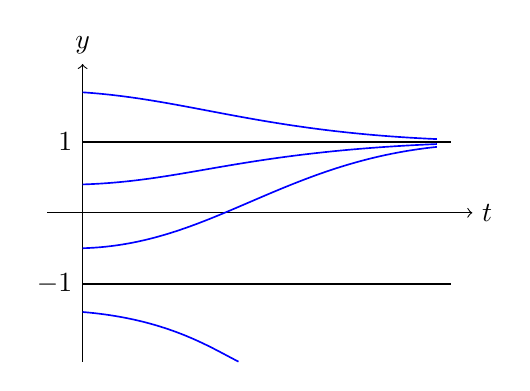
\begin{tikzpicture}[scale=0.9]
		\draw [->] (-0.5, 0) -- (5.5, 0) node [right] {$t$};
		\draw [->] (0, -2.1) -- (0, 2.1) node [above] {$y$};
		\draw [thick] (0, 1) node [left] {$1$} -- (5.2, 1);
		\draw [thick] (0, -1) node [left] {$-1$} -- (5.2, -1);
		\draw [blue, semithick] (0, 0.4) .. controls (1.5, 0.45) and (2.2, 0.85) .. (5, 0.97);
		\draw [blue, semithick] (0, -0.5) .. controls (1.8, -0.45) and (2.8, 0.7) .. (5, 0.93);
		\draw [blue, semithick] (0, 1.7) .. controls (1.5, 1.6) and (2.5, 1.15) .. (5, 1.04);
		\draw [blue, semithick] (0, -1.4) .. controls (1.2, -1.5) and (1.8, -1.9) .. (2.2, -2.1);
	\end{tikzpicture}
	\end{center}

	Note the qualitative structure: $y = 1$ attracts nearby solutions, while $y = -1$ repels them.
\end{example}

\begin{example}[Straight-Line Isoclines]
	Consider $\frac{\mathrm{d}y}{\mathrm{d}x} = x - y$. The isoclines $x - y = D$ are parallel straight lines of unit slope, along which all solution curves have slope $D$. Something special happens on the isocline $x - y = 1$: the prescribed slope there is $1$, which is exactly the slope of the isocline itself -- so that line is \emph{itself a solution}, $y = x - 1$.

	Above this line ($y > x - 1$), slopes are less than $1$; below it, greater than $1$; and one can convince oneself from the slope field that all solutions converge towards the line $y = x - 1$ as $x \to \infty$.

	Since the equation is actually linear, we can confirm this: the integrating factor is $e^x$, giving $(e^x y)' = x e^x$, so $e^x y = (x - 1)e^x + C$ and
	$$
	y = x - 1 + Ce^{-x}.
	$$
	Every solution is the special straight line plus an exponentially decaying correction -- precisely the convergence the isoclines predicted.
\end{example}

\subsection{Equilibrium Points and Stability}

The behaviour in the last example -- solutions being attracted to or repelled from constant solutions -- is so important that it deserves proper terminology.

\begin{definition}[Equilibrium Point]
	An \vocab{equilibrium point} (or \vocab{fixed point}) of a differential equation is a constant solution $y = c$, i.e.\ one with $\frac{\mathrm{d}y}{\mathrm{d}t} = 0$ for all $t$.
\end{definition}

Equilibria are usually the easiest solutions to find: just set the right-hand side of the equation to zero and solve.

\begin{definition}[Stability]
	An equilibrium $y = c$ is \vocab{stable} if whenever $y$ is perturbed slightly from $c$, we have $y \to c$ as $t \to \infty$. It is \vocab{unstable} if small perturbations grow.
\end{definition}

\subsubsection{Perturbation Analysis}

To determine stability we use \emph{perturbation analysis}, which is really just a Taylor expansion. Suppose $y = a$ is a fixed point of $\dot{y} = f(y, t)$, so $f(a, t) = 0$ for all $t$. Set
$$
y(t) = a + \varepsilon(t),
$$
where $\varepsilon$ is a small perturbation. Substituting into the equation and Taylor expanding $f$ in its first argument about $a$:
$$
\dot{\varepsilon} = f(a + \varepsilon, t) = \underbrace{f(a, t)}_{= \, 0} + \, \varepsilon \frac{\partial f}{\partial y}(a, t) + O(\varepsilon^2).
$$
While $\varepsilon$ remains small the $O(\varepsilon^2)$ term is negligible, and we are left with the \vocab{linearised equation}
$$
\dot{\varepsilon} \simeq \varepsilon \, \frac{\partial f}{\partial y}(a, t),
$$
a linear equation which we know how to solve. If the resulting $\varepsilon$ decays, the equilibrium is stable; if it grows, unstable\footnote{Strictly, once $\varepsilon$ has grown large the linearisation is no longer valid, so we cannot conclude that $\varepsilon \to \infty$ -- only that the perturbation initially grows and the solution moves away from the equilibrium. That is exactly what instability means.}.

\begin{example}
	Return to $\dot y = t(1 - y^2)$, with fixed points $y = \pm 1$. We have
	$$
	\frac{\partial f}{\partial y} = -2yt = \begin{cases} -2t & \text{at } y = 1, \\ 2t & \text{at } y = -1. \end{cases}
	$$
	At $y = 1$: $\dot\varepsilon = -2t \varepsilon$, so $\varepsilon = \varepsilon_0 e^{-t^2} \to 0$, and $y = 1$ is stable. At $y = -1$: $\dot\varepsilon = 2t\varepsilon$, so $\varepsilon = \varepsilon_0 e^{t^2}$ grows, and $y = -1$ is unstable -- exactly as our sketch suggested.
\end{example}

\subsubsection{Autonomous Equations and the Phase Line}

Very often the physics of a system doesn't change with time, so that $\dot y$ depends only on $y$ itself.

\begin{definition}[Autonomous Equation]
	An equation of the form $\dot{y} = f(y)$, with no explicit $t$ dependence, is called \vocab{autonomous}.
\end{definition}

For autonomous equations the perturbation analysis is particularly simple. Near a fixed point $y = a$ with $f(a) = 0$, the linearisation is
$$
\dot\varepsilon = f'(a) \, \varepsilon = k \varepsilon \implies \varepsilon = \varepsilon_0 e^{kt},
$$
with $k = f'(a)$ constant. So the rule is simply:
$$
f'(a) < 0 \implies \text{stable}, \qquad f'(a) > 0 \implies \text{unstable}.
$$
Graphically, this is obvious: plot $f(y)$ against $y$. Where $f > 0$, $y$ increases; where $f < 0$, $y$ decreases. So $y$ flows to the right where the graph is above the axis and to the left where it is below, and the fixed points where $f$ crosses the axis \emph{downwards} are the stable ones. Recording just the fixed points and flow directions on a copy of the $y$-axis gives the \vocab{phase portrait} (or phase line) of the equation, a diagram which captures the entire qualitative behaviour at a glance.

\begin{example}[Chemical Kinetics]
	Consider the reaction $\mathrm{NaOH} + \mathrm{HCl} \to \mathrm{NaCl} + \mathrm{H_2O}$, with $a$ molecules of NaOH and $b$ of HCl present, starting from $a_0$ and $b_0$ respectively, and $c$ molecules of each product formed. In dilute solution the reaction rate is proportional to $ab$, so
	$$
	\frac{\mathrm{d}c}{\mathrm{d}t} = \lambda a b = \lambda (a_0 - c)(b_0 - c) = f(c).
	$$
	Suppose (without loss of generality) that $a_0 < b_0$. The graph of $f(c)$ is an upward parabola with roots at $c = a_0$ and $c = b_0$; between the roots $f > 0$, so $c$ increases towards $a_0$ from below. Checking stability: $f'(c) = \lambda(2c - a_0 - b_0)$, so $f'(a_0) = \lambda (a_0 - b_0) < 0$ and $f'(b_0) = \lambda(b_0 - a_0) > 0$. Hence $c = a_0$ is stable and $c = b_0$ is unstable.

	\begin{center}
	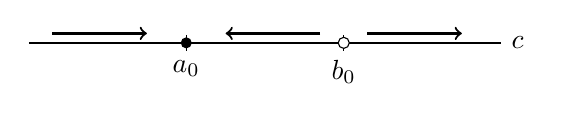
\begin{tikzpicture}
		\draw [thick] (0, 0) -- (6, 0) node [right] {$c$};
		\draw [thick, ->] (0.3, 0.12) -- (1.5, 0.12);
		\draw [thick, ->] (3.7, 0.12) -- (2.5, 0.12);
		\draw [thick, ->] (4.3, 0.12) -- (5.5, 0.12);
		\draw (2, 0.1) -- (2, -0.1) node [below] {$a_0$};
		\draw (4, 0.1) -- (4, -0.1) node [below] {$b_0$};
		\fill (2, 0) circle (2pt);
		\draw [fill=white] (4, 0) circle (2pt);
	\end{tikzpicture}
	\end{center}

	Physically, of course, only $0 \leq c \leq a_0$ makes sense (we cannot have a negative amount of NaOH!), and every physical solution tends to $c = a_0$: the reaction runs until the scarcer reagent is used up.

	For completeness, the equation is separable and can be solved exactly:
	$$
	c = \frac{a_0 b_0 \left[1 - e^{-(b_0 - a_0)\lambda t}\right]}{b_0 - a_0 e^{-(b_0 - a_0)\lambda t}},
	$$
	which indeed tends to $a_0$ as $t \to \infty$ -- but notice how much less work the phase portrait was.
\end{example}

\subsection{The Logistic Equation}

The logistic equation is the classic model of a population limited by finite resources, and it makes a nice showcase for everything in this section.

Consider a population of size $y$ with birth rate $\alpha y$ and death rate $\beta y$. Then $\dot y = (\alpha - \beta) y$, giving exponential growth or decay -- fine for small populations, but unsustainable forever. To model competition for limited resources, note that the rate of pairwise encounters between individuals is proportional to $y^2$, so fighting over scarce food contributes an extra death rate $\gamma y^2$. This gives
$$
\frac{\mathrm{d}y}{\mathrm{d}t} = (\alpha - \beta) y - \gamma y^2 = r y \left(1 - \frac{y}{Y}\right),
$$
where $r = \alpha - \beta$ and $Y = r/\gamma$. This is the \vocab{logistic equation}.

The equation is separable and can be solved explicitly, but the phase portrait tells the whole story with far less effort. Take $r > 0$. The graph of $f(y) = ry(1 - y/Y)$ is a downward parabola with zeros at $y = 0$ and $y = Y$:
\begin{itemize}
	\item $f'(0) = r > 0$, so $y = 0$ is unstable;
	\item $f'(Y) = -r < 0$, so $y = Y$ is stable.
\end{itemize}
For small populations $\dot y \simeq ry$ and growth is exponential; as $y$ approaches the \emph{carrying capacity} $Y$ the growth saturates, and every positive solution tends to $Y$. The characteristic S-shaped (`sigmoid') solution curves interpolate between exponential growth at the bottom and saturation at the top.

For completeness, let's also solve the equation exactly. Separating variables and using partial fractions,
$$
\int \frac{\mathrm{d}y}{y(1 - y/Y)} = \int \left(\frac 1y + \frac{1/Y}{1 - y/Y}\right)\mathrm{d}y = \ln \frac{y}{1 - y/Y} = rt + C,
$$
so $\frac{y}{1 - y/Y} = A e^{rt}$, and solving for $y$ with $y(0) = y_0$:
$$
y(t) = \frac{Y y_0 \, e^{rt}}{Y + y_0(e^{rt} - 1)}.
$$
As a sanity check: for small $t$ (while $y \ll Y$) this is approximately $y_0 e^{rt}$, and as $t \to \infty$ it tends to $Y$, from below if $y_0 < Y$ and from above if $y_0 > Y$ -- exactly the picture the phase portrait predicted, with rather more algebra.

\section{First-Order Difference Equations}

Differential equations describe quantities evolving continuously; but many systems evolve in discrete steps -- populations with annual breeding seasons, and (importantly) any differential equation being solved numerically on a computer. The discrete analogue of a first-order ODE is a \vocab{difference equation} (or \emph{recurrence}, or \emph{map})
$$
x_{n + 1} = f(x_n),
$$
which generates a sequence from a starting value $x_0$. The theory runs parallel to the continuous case, but with some genuine surprises.

\subsection{Fixed Points and Stability}

As with differential equations, the natural starting point is to look for solutions that don't change at all.

\begin{definition}[Fixed Point of a Map]
	A \vocab{fixed point} of $x_{n+1} = f(x_n)$ is a value $x^*$ with $f(x^*) = x^*$, so that the constant sequence $x_n = x^*$ is a solution.
\end{definition}

To analyse stability we perturb, just as before. Write $x_n = x^* + \varepsilon_n$ and expand:
$$
x^* + \varepsilon_{n + 1} = f(x^* + \varepsilon_n) = f(x^*) + \varepsilon_n f'(x^*) + O(\varepsilon_n^2),
$$
so to leading order $\varepsilon_{n+1} \simeq f'(x^*)\, \varepsilon_n$, giving $\varepsilon_n \simeq \varepsilon_0 \, [f'(x^*)]^n$. The perturbation shrinks precisely when the multiplier has modulus less than one:
$$
|f'(x^*)| < 1 \implies \text{stable}, \qquad |f'(x^*)| > 1 \implies \text{unstable}.
$$
Note the contrast with the continuous case, where the criterion was on the \emph{sign} of $f'$; here it is on the \emph{magnitude}. Note also that $f'(x^*)$ negative and small gives \emph{oscillatory} convergence, with the iterates alternating sides of the fixed point.

\begin{remark}[Reconciling the Two Criteria]
	The discrete and continuous stability criteria fit together neatly. The Euler discretisation of $\dot y = f(y)$ with step $h$ is the map $y_{n + 1} = y_n + h f(y_n)$, whose fixed points coincide with the equilibria of the ODE, and whose multiplier there is
	$$
	1 + h f'(a).
	$$
	If $f'(a) < 0$ (stable for the ODE), then for small enough $h$ we have $|1 + hf'(a)| < 1$ and the map is stable too, consistent with the ODE. But if $h > 2/|f'(a)|$, the multiplier drops below $-1$ and the discretisation is unstable even though the ODE is perfectly stable -- a numerical instability caused purely by too large a time step. Numerical analysts spend a great deal of effort designing schemes that avoid this.
\end{remark}

A useful way to visualise iteration is a \vocab{cobweb diagram}: draw the graphs of $x_{n+1} = f(x_n)$ and the diagonal $x_{n + 1} = x_n$, then trace vertically to the curve and horizontally to the diagonal, repeatedly. Fixed points are where curve meets diagonal, and the stability criterion $|f'| < 1$ says the curve crosses the diagonal less steeply than $45\dg$.

\begin{center}
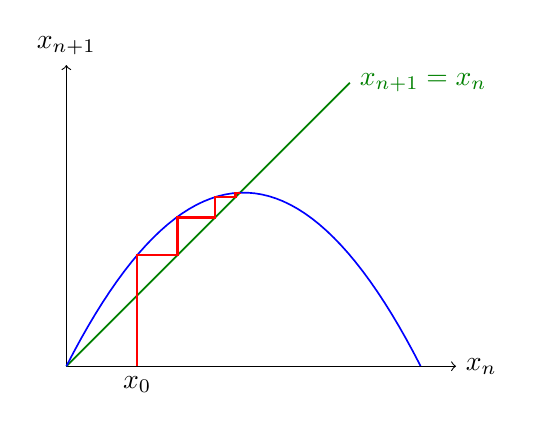
\begin{tikzpicture}[scale=4.5]
	\draw [->] (0, 0) -- (1.1, 0) node [right] {$x_n$};
	\draw [->] (0, 0) -- (0, 0.85) node [above] {$x_{n+1}$};
	\draw [semithick, green!50!black] (0, 0) -- (0.8, 0.8) node [right] {$x_{n+1} = x_n$};
	\draw [semithick, blue, domain=0:1, samples=50] plot (\x, {0.7*2.8*\x*(1-\x)});
	\draw [red, thick] (0.2, 0) node [below, black] {$x_0$}
		-- (0.2, 0.3136) -- (0.3136, 0.3136)
		-- (0.3136, 0.42) -- (0.42, 0.42)
		-- (0.42, 0.4772) -- (0.4772, 0.4772)
		-- (0.4772, 0.4885) -- (0.4885, 0.4885)
		-- (0.4885, 0.4897) -- (0.4897, 0.4897);
\end{tikzpicture}
\end{center}

(The cobweb above shows convergence towards a stable fixed point where the blue curve cuts the diagonal.)

\subsection{The Logistic Map}

Discretising the logistic equation with the Euler scheme (time step $\Delta t$):
$$
\frac{y_{n + 1} - y_n}{\Delta t} = r y_n \left(1 - \frac{y_n}{Y}\right),
$$
and rescaling via $\lambda = 1 + r \Delta t$ and $x_n = \frac{r \Delta t}{1 + r\Delta t} \cdot \frac{y_n}{Y}$, one arrives (after a little algebra) at the famous \vocab{logistic map}
$$
x_{n + 1} = \lambda x_n (1 - x_n).
$$
Its fixed points satisfy $\lambda x(1 - x) = x$, giving
$$
x^* = 0 \qquad \text{or} \qquad x^* = 1 - \frac{1}{\lambda},
$$
and $f'(x) = \lambda(1 - 2x)$, so $f'(0) = \lambda$ and $f'(1 - 1/\lambda) = 2 - \lambda$. The stability analysis then predicts strikingly rich behaviour as $\lambda$ increases:
\begin{enumerate}[label=(\roman*)]
	\item For $0 < \lambda < 1$: only $x^* = 0$ is relevant, $|f'(0)| = \lambda< 1$, and the population dies out.
	\item For $1 < \lambda < 2$: $x^* = 0$ becomes unstable, and $x^* = 1 - 1/\lambda$ is stable with $0 < f' < 1$, so iterates converge to it monotonically.
	\item For $2 < \lambda < 3$: still stable, but now $-1 < f' < 0$, so the convergence is oscillatory, with iterates spiralling into the fixed point on the cobweb diagram.
	\item For $\lambda > 3$: $|f'(x^*)| > 1$, so \emph{both} fixed points are unstable. The iterates settle instead into a \emph{2-cycle}, oscillating between two values (a solution of $x_{n+2} = x_n$). As $\lambda$ increases further to $1 + \sqrt 6 \approx 3.449$, the 2-cycle destabilises in favour of a 4-cycle, then an 8-cycle, and so on -- a \emph{period-doubling cascade} which accumulates at $\lambda \approx 3.57$, beyond which the dynamics become chaotic.
\end{enumerate}
The moral is worth remembering: a discretisation can have wildly different behaviour from the differential equation it approximates. The continuous logistic equation is completely tame -- every positive solution glides monotonically to the carrying capacity -- while its discrete counterpart, for large enough $\lambda$ (i.e.\ large enough time step), is chaotic.

\section{Second-Order Linear Differential Equations}

We now move up an order. Second-order linear equations are probably the most important differential equations in all of physics -- Newton's second law is one -- and they will occupy us for a good while. Almost everything we do in this section extends routinely to higher-order linear equations, but second order is where all the ideas already appear.

\subsection{Constant Coefficients and the Characteristic Equation}

The general second-order linear equation with constant coefficients is
$$
a y'' + b y' + c y = f(x).
$$
Following the strategy from the first-order case, we solve this in two steps: find the general solution of the homogeneous equation $ay'' + by' + cy = 0$ (the complementary function), then find any one particular integral of the full equation, and add them.

For the complementary function, we again exploit the fact that $e^{\lambda x}$ is an eigenfunction of $\frac{\mathrm{d}}{\mathrm{d}x}$, and hence also of $\frac{\mathrm{d}^2}{\mathrm{d}x^2}$. Trying $y = e^{\lambda x}$ gives $a\lambda^2 e^{\lambda x} + b \lambda e^{\lambda x} + c e^{\lambda x} = 0$, and dividing by the (never-zero) exponential:

\begin{definition}[Characteristic Equation]
	The \vocab{characteristic equation} of $ay'' + by' + cy = 0$ is
	$$
	a\lambda^2 + b\lambda + c = 0.
	$$
\end{definition}

This is a quadratic with two roots $\lambda_1, \lambda_2$. If they are distinct, we get two genuinely different solutions $e^{\lambda_1 x}$ and $e^{\lambda_2 x}$, and (as we will justify carefully in \S\ref{sec:phase-space}) the general complementary function is
$$
y_c = A e^{\lambda_1 x} + B e^{\lambda_2 x}.
$$

\begin{example}
	Consider $y'' - 5y' + 6y = 0$. The characteristic equation is $\lambda^2 - 5\lambda + 6 = 0$, with roots $\lambda = 2, 3$. So the general solution is
	$$
	y = A e^{2x} + B e^{3x}.
	$$
\end{example}

\begin{example}[Simple Harmonic Motion]
	Consider $y'' + 4y = 0$. The characteristic equation is $\lambda^2 + 4 = 0$, so $\lambda = \pm 2i$ and
	$$
	y = A e^{2ix} + B e^{-2ix}.
	$$
	The constants $A, B$ are allowed to be complex, but if this is modelling a physical oscillation we would like the answer to at least \emph{look} real. Expanding with Euler's formula,
	$$
	y = A(\cos 2x + i \sin 2x) + B (\cos 2x - i \sin 2x) = \alpha \cos 2x + \beta \sin 2x,
	$$
	where $\alpha = A + B$ and $\beta = i(A - B)$. All we have done is change basis for the solution space, from $\{e^{2ix}, e^{-2ix}\}$ to $\{\cos 2x, \sin 2x\}$; whichever basis is more convenient may be used. More generally, complex roots $\lambda = \sigma \pm i\omega$ give solutions $e^{\sigma x}(\alpha \cos \omega x + \beta \sin \omega x)$ -- oscillations with exponentially growing or decaying amplitude.
\end{example}

\begin{remark}[Higher-Order Equations]
	Everything here generalises immediately: an $n$th-order linear equation with constant coefficients has characteristic polynomial of degree $n$, and each distinct root $\lambda$ contributes $e^{\lambda x}$ to the complementary function. For example, radioactive decay \emph{sequences} $A \to B \to C \to \cdots$, which we treated one step at a time in the previous section, can be packaged as a single higher-order equation whose characteristic roots are $-k_a, -k_b, -k_c, \dots$ -- each isotope contributing its own decaying exponential to the mix.
\end{remark}

\subsection{Degeneracy and Detuning}

Something goes wrong when the characteristic equation has a repeated root: our method produces only \emph{one} solution, but a second-order equation should have a two-parameter family.

\begin{example}[A Repeated Root]
	Consider $y'' - 4y' + 4y = 0$. The characteristic equation is $(\lambda - 2)^2 = 0$, so $\lambda = 2$ twice, and we find only the single solution family $Ae^{2x}$. The solution space is two-dimensional, so we are missing a second, independent solution.

	Here is a rather beautiful way of finding it, called \vocab{detuning}. The problem is that our two roots collided, so let's separate them slightly: perturb the equation to
	$$
	y'' - 4y' + (4 - \varepsilon^2) y = 0,
	$$
	which has roots $\lambda = 2 \pm \varepsilon$, and recovers our equation as $\varepsilon \to 0$. For $\varepsilon \neq 0$ the general solution is
	$$
	y = A e^{(2 + \varepsilon)x} + B e^{(2 - \varepsilon)x} = e^{2x}\left[A e^{\varepsilon x} + B e^{-\varepsilon x}\right].
	$$
	Now Taylor expand the small exponentials:
	$$
	y = e^{2x}\left[(A + B) + \varepsilon x (A - B) + O(\varepsilon^2 A, \varepsilon^2 B)\right].
	$$
	Fix constants $\alpha$ and $\beta$, and for each small $\varepsilon$ choose $A = \frac{1}{2}(\alpha + \beta/\varepsilon)$ and $B = \frac{1}{2}(\alpha - \beta/\varepsilon)$, so that $A + B = \alpha$ and $\varepsilon(A - B) = \beta$. Since $A, B = O(1/\varepsilon)$, the error terms are $O(\varepsilon)$, and letting $\varepsilon \to 0$,
	$$
	y \to e^{2x} (\alpha + \beta x).
	$$
	So the missing second solution is $x e^{2x}$.
\end{example}

The pattern in this example is completely general, and worth committing to memory: \emph{if the characteristic equation has a repeated root $\lambda$, the complementary function is $(A + Bx)e^{\lambda x}$}.

\subsection{Reduction of Order}

Detuning relied on constant coefficients. There is a more robust technique for manufacturing a second solution out of a known one, which works for any linear second-order equation: look for a solution of the form
$$
y_2(x) = v(x) \, y_1(x),
$$
where $y_1$ is the solution we already have and $v$ is to be found. The point is that substituting this in always produces a \emph{first-order} equation for $v'$ (the $v$ terms cancel because $y_1$ is a solution) -- hence the name \vocab{reduction of order}.

\begin{example}
	Take $y'' - 4y' + 4y = 0$ again, with known solution $y_1 = e^{2x}$. Try $y_2 = v e^{2x}$. Then
	$$
	y_2' = (v' + 2v)e^{2x}, \qquad y_2'' = (v'' + 4v' + 4v)e^{2x},
	$$
	and substituting in,
	$$
	\left[(v'' + 4v' + 4v) - 4(v' + 2v) + 4v\right]e^{2x} = 0 \implies v'' = 0.
	$$
	So $v = Ax + B$, and $y_2 = (Ax + B)e^{2x}$ -- recovering the answer from detuning, this time with essentially no cleverness required.
\end{example}

\subsection{Phase Space, Linear Independence and the Wronskian}\label{sec:phase-space}

We have been asserting that a second-order linear equation has a two-parameter family of solutions, and that certain pairs of solutions are `independent'. Let's now make this precise.

Consider a general $n$th-order linear equation. Its solution is not determined by the value $y(x_0)$ alone: we also need $y'(x_0)$, and so on up to $y^{(n-1)}(x_0)$. Once these $n$ numbers are known, the equation itself determines $y^{(n)}(x_0)$, and by differentiating the equation, all higher derivatives too -- so the entire Taylor series of the solution at $x_0$ is pinned down. This strongly suggests (and it is true, though a real proof needs the machinery of IB Analysis) that a solution is uniquely determined by the $n$ initial conditions $y(x_0), y'(x_0), \dots, y^{(n-1)}(x_0)$.

This motivates packaging those numbers into a single object.

\begin{definition}[Solution Vector and Phase Space]
	The \vocab{solution vector} of a solution $y$ of an $n$th-order differential equation is
	$$
	\vv{Y}(x) = \left(y(x), y'(x), \dots, y^{(n - 1)}(x)\right).
	$$
	The $n$-dimensional space in which $\vv{Y}$ lives is called \vocab{phase space}. As $x$ varies, $\vv{Y}(x)$ traces out a \vocab{trajectory} in phase space, and each point of phase space (viewed as an initial condition) has a unique trajectory through it.
\end{definition}

\begin{example}
	Consider $y'' + 4y = 0$. The initial condition $y(0) = 1$, $y'(0) = 0$ gives the solution $y_1 = \cos 2x$, with solution vector $\vv{Y}_1(x) = (\cos 2x, -2\sin 2x)$ -- which traces out an ellipse in phase space, traversed clockwise. The initial condition $y(0) = 0$, $y'(0) = 2$ gives $y_2 = \sin 2x$, with $\vv{Y}_2(x) = (\sin 2x, 2\cos 2x)$.

	Notice that the two initial vectors $(1, 0)$ and $(0, 2)$ are linearly independent, and one can check that $\vv{Y}_1(x)$ and $\vv{Y}_2(x)$ remain linearly independent for \emph{every} $x$. This is not a coincidence, as we will now see.
\end{example}

For a second-order equation, phase space is a plane, and a natural question is whether two solutions $y_1, y_2$ give solution vectors forming a basis of that plane. The determinant testing this has a name.

\begin{definition}[Wronskian]
	The \vocab{Wronskian} of two solutions $y_1, y_2$ of a second-order differential equation is the determinant
	$$
	W(x) = \begin{vmatrix} y_1 & y_2 \\ y_1' & y_2' \end{vmatrix} = y_1 y_2' - y_2 y_1'.
	$$
\end{definition}

\begin{definition}[Independent Solutions]
	Solutions $y_1$ and $y_2$ are \vocab{independent} if their solution vectors $\vv{Y}_1(x), \vv{Y}_2(x)$ are linearly independent for some $x$ -- that is, if $W(x) \neq 0$ for some $x$.
\end{definition}

\begin{example}
	For $y'' + 4y = 0$ with $y_1 = \cos 2x$, $y_2 = \sin 2x$:
	$$
	W = \cos 2x \cdot 2 \cos 2x - \sin 2x \cdot (-2 \sin 2x) = 2 \neq 0.
	$$
	For $y'' - 4y' + 4y = 0$ with $y_1 = e^{2x}$, $y_2 = x e^{2x}$:
	$$
	W = \begin{vmatrix} e^{2x} & x e^{2x} \\ 2e^{2x} & (1 + 2x) e^{2x}\end{vmatrix} = e^{4x}(1 + 2x - 2x) = e^{4x} \neq 0.
	$$
\end{example}

In both examples the Wronskian was non-vanishing \emph{everywhere}. Could the Wronskian vanish at some points but not others? Remarkably, no.

\begin{theorem}[Abel's Theorem]
	Let $y_1, y_2$ be solutions of $y'' + p(x) y' + q(x) y = 0$. Then either $W \equiv 0$, or $W(x) \neq 0$ for all $x$. In particular, if two solutions are independent at one point, they are independent everywhere.
\end{theorem}
\begin{proof}
	Since $y_1$ and $y_2$ are both solutions,
	\begin{align*}
		y_2 (y_1'' + p y_1' + q y_1) &= 0, \\
		y_1 (y_2'' + p y_2' + q y_2) &= 0.
	\end{align*}
	Subtracting the first from the second,
	$$
	(y_1 y_2'' - y_2 y_1'') + p (y_1 y_2' - y_2 y_1') = 0.
	$$
	Now observe that $W = y_1 y_2' - y_2 y_1'$ and, differentiating, $W' = y_1 y_2'' - y_2 y_1''$ (the cross terms cancel). So the equation above says precisely
	$$
	W' + p(x) W = 0,
	$$
	a first-order linear equation for $W$, with solution
	$$
	W(x) = W_0 \, e^{-\int p \dd x}.
	$$
	Since the exponential never vanishes, either $W_0 = 0$ and $W \equiv 0$, or $W$ is nowhere zero.
\end{proof}

\begin{remark}
	Abel's theorem generalises: writing an $n$th-order homogeneous linear equation as a first-order system $\vv{Y}' = A \vv{Y}$ (as we will do in \S\ref{sec:systems}), one can show $W' + \tr(A) W = 0$, so $W = W_0 e^{-\int \tr A \dd x}$ and the same dichotomy holds.
\end{remark}

\subsection{Particular Integrals}

With the complementary function understood, we return to the forced equation
$$
a y'' + by' + cy = f(x)
$$
and the problem of finding a particular integral. The first method, as ever, is educated guessing: choose a trial form matching the forcing, with unknown coefficients, and substitute. The standard guesses are:
\begin{center}
	\begin{tabular}{cc}
		$f(x)$ & trial $y_p(x)$ \\[2pt]
		\hline \\[-8pt]
		$e^{mx}$ & $A e^{mx}$ \\
		$\sin kx$ or $\cos kx$ & $A \sin kx + B \cos kx$ \\
		polynomial of degree $n$ & $a_n x^n + \cdots + a_1 x + a_0$
	\end{tabular}
\end{center}
Note that for trigonometric forcing we must include \emph{both} $\sin$ and $\cos$ in the guess (differentiation mixes them), and for polynomial forcing all lower-order terms. Since the equation is linear, a sum of forcing terms can be handled term by term and the particular integrals superposed.

\begin{example}
	Consider $y'' - 5y' + 6y = 2x + e^{4x}$. We guess $y_p = ax + b + ce^{4x}$. Then $y_p' = a + 4ce^{4x}$ and $y_p'' = 16 c e^{4x}$, and substituting in:
	$$
	16 c e^{4x} - 5(a + 4ce^{4x}) + 6(ax + b + ce^{4x}) = 2x + e^{4x}.
	$$
	Comparing coefficients of $e^{4x}$, $x$ and $1$ respectively:
	\begin{align*}
		16c - 20c + 6c = 1 &\implies c = \tfrac{1}{2}, \\
		6a = 2 &\implies a = \tfrac{1}{3}, \\
		-5a + 6b = 0 &\implies b = \tfrac{5}{18}.
	\end{align*}
	The complementary function was found earlier, so the general solution is
	$$
	y = A e^{3x} + B e^{2x} + \frac{1}{2}e^{4x} + \frac{1}{3}x + \frac{5}{18}.
	$$
\end{example}

\subsection{Resonance}

The guessing procedure breaks down in one important situation: when the forcing is itself a complementary function.

Consider a simple harmonic oscillator forced at its own natural frequency:
$$
\ddot{y} + \omega_0^2 y = \sin \omega_0 t.
$$
The complementary function is $y_c = A \sin \omega_0 t + B \cos \omega_0 t$, and if we try $y_p = C \sin \omega_0 t + D \cos \omega_0 t$, we just get $\ddot y_p + \omega_0^2 y_p = 0$ -- the guess is annihilated by the operator, and can never balance the forcing. This phenomenon is called \vocab{resonance}.

To understand what actually happens, we detune again: force at a nearby frequency $\omega \neq \omega_0$,
$$
\ddot y + \omega_0^2 y = \sin \omega t,
$$
and take the limit $\omega \to \omega_0$ at the end. Guessing the antisymmetric combination $y_p = C(\sin \omega t - \sin \omega_0 t)$ (chosen so that $y_p \to 0$ as $\omega \to \omega_0$, keeping the limit finite), we have
$$
\ddot y_p = C(-\omega^2 \sin \omega t + \omega_0^2 \sin \omega_0 t),
$$
and substituting in gives $C(\omega_0^2 - \omega^2) = 1$. So
$$
y_p = \frac{\sin \omega t - \sin \omega_0 t}{\omega_0^2 - \omega^2} = \frac{2}{\omega_0^2 - \omega^2} \cos\left(\frac{\omega_0 + \omega}{2} t\right) \sin \left(\frac{\omega - \omega_0}{2}t\right),
$$
using the sum-to-product formula. Writing $\Delta \omega = \omega_0 - \omega$, this is a fast oscillation at roughly the natural frequency, modulated by a slow envelope $\sin(\Delta\omega \, t/2)$ of amplitude $O(1/\Delta \omega)$ and period $O(1/\Delta\omega)$. This slow waxing and waning of amplitude, familiar from tuning musical instruments, is called \vocab{beating}: it occurs whenever a system is forced close to (but not exactly at) its natural frequency.

Now let $\Delta \omega \to 0$. The envelope's wavelength stretches to infinity, and using $\sin \theta \approx \theta$ for the slow factor,
$$
y_p \to -\frac{t}{2\omega_0} \cos \omega_0 t.
$$
So at exact resonance, the response is an oscillation whose amplitude \emph{grows linearly in time} -- the initial stretch of linear growth is all that remains of the beat envelope. This also tells us the correct guess to make at resonance, and the rule is general: \emph{if the forcing is a complementary function, multiply the usual guess by the independent variable}. (If that is somehow still a complementary function, multiply by it again.)

\begin{example}
	For $\ddot y + \omega_0^2 y = \sin \omega_0 t$, try $y_p = t(C \sin \omega_0 t + D \cos \omega_0 t)$. Substituting in, the $t$-proportional terms cancel (as they must -- they are complementary functions) leaving
	$$
	2 C \omega_0 \cos \omega_0 t - 2D\omega_0 \sin \omega_0 t = \sin \omega_0 t,
	$$
	so $C = 0$, $D = -1/(2\omega_0)$, and $y_p = -\frac{t}{2\omega_0}\cos \omega_0 t$, in agreement with the limit above.
\end{example}

\subsection{Variation of Parameters}

Guessing works when the forcing is simple. \vocab{Variation of parameters} is a systematic method that works for \emph{any} forcing, provided we know the complementary functions. It is more work than guessing, so it should be a last resort -- but it always succeeds.

Consider
$$
y'' + p(x) y' + q(x) y = f(x),
$$
with independent complementary functions $y_1, y_2$. The idea comes from phase space: for each fixed $x$, the solution vectors $\vv{Y}_1(x)$ and $\vv{Y}_2(x)$ form a basis of the plane, so the particular solution vector we seek can be expanded in that basis, with coefficients that vary with $x$:
$$
\vv{Y}_p(x) = u(x) \vv{Y}_1(x) + v(x) \vv{Y}_2(x).
$$
Reading off the two components,
\begin{align}
	y_p &= u y_1 + v y_2, \tag{a} \\
	y_p' &= u y_1' + v y_2'. \tag{b}
\end{align}
These two equations carry a hidden constraint: differentiating (a) gives $y_p' = uy_1' + vy_2' + u'y_1 + v'y_2$, which is consistent with (b) only if
\begin{equation}
u' y_1 + v' y_2 = 0. \tag{c}
\end{equation}
Now differentiate (b):
$$
y_p'' = u y_1'' + v y_2'' + u' y_1' + v' y_2',
$$
and substitute everything into the differential equation. The terms multiplying $u$ and $v$ vanish (since $y_1, y_2$ are complementary functions), leaving
\begin{equation}
u' y_1' + v' y_2' = f. \tag{d}
\end{equation}
Equations (c) and (d) are two linear equations for $u'$ and $v'$:
$$
\begin{pmatrix} y_1 & y_2 \\ y_1' & y_2' \end{pmatrix}
\begin{pmatrix} u' \\ v' \end{pmatrix} = \begin{pmatrix} 0 \\ f \end{pmatrix},
$$
and the matrix is invertible precisely because its determinant is the Wronskian $W \neq 0$. Inverting,
$$
u' = -\frac{y_2 f}{W}, \qquad v' = \frac{y_1 f}{W},
$$
and integrating gives $u$ and $v$, hence $y_p$. (It is far better to remember the derivation than the formula.)

\begin{example}
	Let's redo resonance by this method: $y'' + 4y = \sin 2x$, with $y_1 = \sin 2x$, $y_2 = \cos 2x$ and $W = y_1y_2' - y_2 y_1' = -2$. Then
	$$
	u' = \frac{\cos 2x \sin 2x}{2} = \frac{\sin 4x}{4}, \qquad v' = -\frac{\sin^2 2x}{2} = \frac{\cos 4x - 1}{4},
	$$
	so
	$$
	u = -\frac{\cos 4x}{16}, \qquad v = \frac{\sin 4x}{16} - \frac{x}{4}.
	$$
	Therefore
	$$
	y_p = \frac{1}{16}\left(-\cos 4x \sin 2x + \sin 4x \cos 2x\right) - \frac{x}{4}\cos 2x = \frac{1}{16}\sin 2x - \frac{x}{4}\cos 2x.
	$$
	The term $-\frac{x}{4}\cos 2x$ is the resonant response we found by detuning (here $\omega_0 = 2$), and $\frac{1}{16}\sin 2x$ is merely a complementary function, so the answers agree.
\end{example}

\begin{example}[When Guessing is Hopeless]
	Consider $y'' + y = \tan x$. No finite combination of elementary functions suggests itself as a guess -- differentiating $\tan x$ generates ever more complicated expressions -- so variation of parameters is the way forward. With $y_1 = \sin x$, $y_2 = \cos x$ and $W = \sin x \cdot(-\sin x) - \cos x \cdot \cos x = -1$:
	$$
	u' = -\frac{y_2 f}{W} = \cos x \tan x = \sin x, \qquad v' = \frac{y_1 f}{W} = -\sin x \tan x = \cos x - \sec x,
	$$
	where we wrote $-\sin^2 x/\cos x = (\cos^2 x - 1)/\cos x$. Integrating,
	$$
	u = -\cos x, \qquad v = \sin x - \ln|\sec x + \tan x|,
	$$
	so
	$$
	y_p = u y_1 + v y_2 = -\cos x \sin x + \sin x \cos x - \cos x \ln |\sec x + \tan x| = -\cos x \ln|\sec x + \tan x|.
	$$
	The general solution is $y = A \sin x + B \cos x - \cos x \ln |\sec x + \tan x|$ -- involving a logarithm that no reasonable person would have guessed.
\end{example}

\subsection{Equidimensional Equations}

There is one important class of \emph{non}-constant coefficient equations that we can solve just as easily.

\begin{definition}[Equidimensional Equation]
	An equation is \vocab{equidimensional} if it has the form
	$$
	a x^2 y'' + b x y' + c y = f(x),
	$$
	with $a, b, c$ constants.
\end{definition}

The name comes from dimensional analysis: if $x$ carries some physical dimension, then each of $x^2 y''$, $xy'$ and $y$ has the same dimensions, so the equation is invariant under rescaling $x \mapsto \lambda x$. (These are often called `homogeneous' equations, but that clashes horribly with our earlier usage, so we avoid it.)

Just as $e^{\lambda x}$ is the eigenfunction of $\frac{\mathrm{d}}{\mathrm{d}x}$, the powers $x^k$ are eigenfunctions of the operator $x \frac{\mathrm{d}}{\mathrm{d}x}$, and this suggests trying $y = x^k$. Since $xy' = k x^k$ and $x^2 y'' = k(k-1)x^k$, substituting into the homogeneous equation gives
$$
a k (k - 1) + bk + c = 0,
$$
with roots $k_1, k_2$, and complementary function $y_c = A x^{k_1} + B x^{k_2}$ when the roots are distinct.

Alternatively, substituting $z = \ln x$ transforms the equation into one with constant coefficients:
$$
a \frac{\mathrm{d}^2 y}{\mathrm{d}z^2} + (b - a) \frac{\mathrm{d}y}{\mathrm{d}z} + c y = f(e^z),
$$
whose characteristic equation $a\lambda(\lambda - 1) + b\lambda + c = 0$ is precisely the one above. This substitution is the easiest way to deal with the degenerate cases: a repeated root $k$ gives $y_c = (A + B \ln x)x^k$ (from $(A + Bz)e^{kz}$), and resonant forcing proportional to $x^{k_1}$ gives a particular integral proportional to $x^{k_1} \ln x$.

\begin{example}
	Let's solve $x^2 y'' - 3xy' + 4y = x^2$ for $x > 0$. Trying $y = x^k$ in the homogeneous equation:
	$$
	k(k - 1) - 3k + 4 = k^2 - 4k + 4 = (k - 2)^2 = 0,
	$$
	a repeated root $k = 2$. So the complementary function is
	$$
	y_c = (A + B \ln x)\, x^2.
	$$
	The forcing $x^2$ is resonant (it is a complementary function!), so following the rule above we try $y_p = C x^2 (\ln x)^2$ -- the usual resonant guess $x^2 \ln x$ is \emph{also} a complementary function here, so we multiply by $\ln x$ once more. Substituting (a slightly tedious computation, best done via $z = \ln x$, where the equation becomes $\frac{\mathrm{d}^2y}{\mathrm{d}z^2} - 4\frac{\mathrm{d}y}{\mathrm{d}z} + 4y = e^{2z}$ with double-resonant forcing and trial $Cz^2 e^{2z}$):
	$$
	C\left(2 + 8z + 4z^2 - 8z - 8z^2 + 4z^2\right)e^{2z} = e^{2z} \implies 2C = 1,
	$$
	so $C = \frac12$ and the general solution is
	$$
	y = \left(A + B \ln x + \tfrac{1}{2}(\ln x)^2\right) x^2.
	$$
\end{example}

\subsection{Transients and Damping}

Let's use what we have built to study a genuinely physical system: a damped, forced oscillator. Consider a car of mass $M$ riding on suspension; the springs supply a restoring force $kx$ and the shock absorbers a friction force $l \dot x$ opposing motion, while $F(t)$ is an external vertical force. Newton's second law gives
$$
M \ddot x = F(t) - kx - l \dot x \implies \ddot x + \frac{l}{M} \dot x + \frac{k}{M} x = \frac{F(t)}{M}.
$$
Without damping and forcing this would be simple harmonic motion with angular frequency $\sqrt{k/M}$. It is illuminating to non-dimensionalise: measure time in units of $\sqrt{M/k}$ by setting $t = \tau \sqrt{M/k}$. The equation becomes
$$
\ddot x + 2\kappa \dot x + x = f(\tau),
$$
where now dots denote $\mathrm{d}/\mathrm{d}\tau$, and
$$
\kappa = \frac{l}{2\sqrt{kM}}, \qquad f = \frac{F}{k}.
$$
The original three parameters $M, l, k$ have collapsed into the single dimensionless damping parameter $\kappa$ -- this sort of reduction is one of the main payoffs of non-dimensionalisation.

Consider first the free response, $f = 0$. The characteristic equation $\lambda^2 + 2\kappa \lambda + 1 = 0$ has roots
$$
\lambda = -\kappa \pm \sqrt{\kappa^2 - 1},
$$
and the character of the motion depends entirely on where $\kappa$ sits relative to $1$.

\begin{enumerate}[label=(\roman*)]
	\item \emph{Underdamped} ($\kappa < 1$). The roots are complex, $\lambda = -\kappa \pm i \sqrt{1 - \kappa^2}$, and
	$$
	x = e^{-\kappa \tau}\left(A \sin \sqrt{1 - \kappa^2}\, \tau + B \cos \sqrt{1 - \kappa^2}\,\tau\right).
	$$
	The system oscillates with period $2\pi/\sqrt{1 - \kappa^2}$ -- note that damping \emph{lengthens} the period -- inside an envelope decaying over a timescale $O(1/\kappa)$. As $\kappa \to 1$ the period tends to infinity.
	\begin{center}
	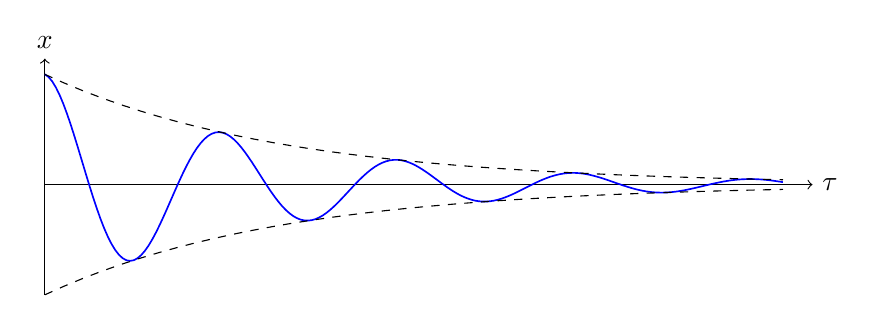
\begin{tikzpicture}[xscale=0.75]
		\draw [->] (0, 0) -- (13, 0) node [right] {$\tau$};
		\draw [->] (0, -1.4) -- (0, 1.6) node [above] {$x$};
		\draw [blue, semithick, domain=0:12.5, samples=200] plot (\x, {1.4*exp(-0.25*\x)*cos(120*\x)});
		\draw [dashed] plot [domain=0:12.5, samples=40] (\x, {1.4*exp(-0.25*\x)});
		\draw [dashed] plot [domain=0:12.5, samples=40] (\x, {-1.4*exp(-0.25*\x)});
	\end{tikzpicture}
	\end{center}
	\item \emph{Critically damped} ($\kappa = 1$). Repeated root $\lambda = -1$, so
	$$
	x = (A + B\tau) e^{-\tau}.
	$$
	The solution can rise at most once before decaying; both the rise and decay happen on the $O(1)$ timescale (i.e.\ $O(\sqrt{M/k})$ in dimensional terms).
	\item \emph{Overdamped} ($\kappa > 1$). Two real negative roots $-\lambda_1 > -\lambda_2$, and
	$$
	x = A e^{-\lambda_1 \tau} + B e^{-\lambda_2 \tau}, \qquad \lambda_{1,2} = \kappa \mp \sqrt{\kappa^2 - 1}.
	$$
	The fast mode dies on a timescale $O(1/\lambda_2)$, and the solution then decays slowly, on the long timescale $O(1/\lambda_1)$. Heavy damping makes the system \emph{slower} to settle.
\end{enumerate}
For car suspension we would tune $\kappa$ close to critical damping: strong enough to kill oscillations, not so strong that the car takes forever to level out.

\begin{example}[An Underdamped Oscillator]
	Let's solve a concrete initial value problem:
	$$
	\ddot x + 2\dot x + 5x = 0, \qquad x(0) = 1, \quad \dot x(0) = 0.
	$$
	The characteristic equation $\lambda^2 + 2\lambda + 5 = 0$ gives $\lambda = -1 \pm 2i$, so
	$$
	x = e^{-t}(A\cos 2t + B \sin 2t).
	$$
	The condition $x(0) = 1$ gives $A = 1$; then $\dot x = e^{-t}\left[(-A + 2B)\cos 2t + (-B - 2A)\sin 2t\right]$, and $\dot x(0) = 0$ gives $B = \frac12$. So
	$$
	x = e^{-t}\left(\cos 2t + \tfrac12 \sin 2t\right),
	$$
	a decaying oscillation: the mass overshoots the origin, swings back, and each successive swing is smaller by a factor $e^{-\pi} \approx 0.04$ (one half-period is $\pi/2$, so a full period costs $e^{-\pi}$ in amplitude). Within a few swings the motion is imperceptible.
\end{example}

Now switch the forcing on, say $f(\tau) = \sin \tau$. In all three cases the roots of the characteristic equation have negative real part, so the complementary function decays exponentially: it is a \vocab{transient}, describing the system's short-time adjustment to its initial conditions. What survives at large times is the particular integral, the \emph{steady-state response}. Guessing $x_p = C \sin \tau + D \cos \tau$ and substituting into $\ddot x + 2\kappa \dot x + x = \sin \tau$:
$$
(-C - 2\kappa D + C) \sin \tau + (-D + 2\kappa C + D) \cos \tau = \sin \tau,
$$
so $C = 0$ and $D = -1/(2\kappa)$, giving
$$
x \sim -\frac{1}{2\kappa} \cos \tau \quad \text{as } \tau \to \infty.
$$
Notice that the long-time response is $90\dg$ out of phase with the forcing (and its amplitude blows up as $\kappa \to 0$ -- our old friend resonance, since the forcing here is at the natural frequency).

\section{Second-Order Difference Equations}

Just as first-order ODEs had discrete analogues, so do second-order equations. Consider
$$
a\, y_{n + 2} + b \, y_{n + 1} + c\, y_n = f_n.
$$
The whole solution theory transfers almost verbatim from the continuous setting, because the same structural facts hold: the equation is linear, and we know an eigenfunction of the basic operator. Here the basic operator is the \emph{shift} $D[y_n] = y_{n + 1}$, and its eigenfunctions are the geometric sequences $y_n = k^n$, since $D[k^n] = k \cdot k^n$.

So, to solve the homogeneous equation $a y_{n+2} + by_{n+1} + cy_n = 0$, we try $y_n = k^n$:
$$
a k^{n + 2} + b k^{n+1} + c k^n = 0 \implies ak^2 + bk + c = 0.
$$
If the roots $k_1, k_2$ are distinct, the general complementary function is
$$
y_n^{(c)} = A k_1^n + B k_2^n,
$$
and if they coincide, $y_n^{(c)} = (A + Bn)k^n$ -- multiplication by $n$ playing exactly the role that multiplication by $x$ played before.

For particular integrals we guess, following the same principles:
\begin{center}
	\begin{tabular}{cc}
		$f_n$ & trial $y_n^{(p)}$ \\[2pt]
		\hline \\[-8pt]
		$k^n$ ($k \neq k_1, k_2$) & $A k^n$ \\
		$k_1^n$ & $A n k_1^n$ \\
		$n^p$ & $A n^p + B n^{p - 1} + \cdots + C$
	\end{tabular}
\end{center}
with the resonant case again handled by an extra factor of $n$.

\begin{example}[The Fibonacci Sequence]
	The Fibonacci numbers satisfy
	$$
	y_{n + 2} - y_{n + 1} - y_n = 0, \qquad y_0 = y_1 = 1.
	$$
	Trying $y_n = k^n$ gives $k^2 - k - 1 = 0$, so
	$$
	k = \frac{1 \pm \sqrt 5}{2}.
	$$
	Write $\varphi_1 = \frac{1 + \sqrt 5}{2}$ (the golden ratio) and $\varphi_2 = \frac{1 - \sqrt{5}}{2}$; note $\varphi_1 \varphi_2 = -1$. The general solution is $y_n = A \varphi_1^n + B\varphi_2^n$, and the initial conditions give
	$$
	A + B = 1, \qquad A \varphi_1 + B \varphi_2 = 1,
	$$
	from which $A = \varphi_1/\sqrt 5$ and $B = -\varphi_2/\sqrt{5}$. Hence
	$$
	y_n = \frac{\varphi_1^{n + 1} - \varphi_2^{n + 1}}{\sqrt 5}.
	$$
	Since $|\varphi_2| < 1$, the second term rapidly becomes negligible: the Fibonacci numbers grow like $\varphi_1^{n+1}/\sqrt 5$, and the ratio of successive terms tends to the golden ratio. (It is mildly miraculous that this expression, stuffed full of $\sqrt 5$'s, is an integer for every $n$ -- but of course it must be.)
\end{example}

\begin{example}[A Forced Difference Equation]
	Consider
	$$
	y_{n + 2} - 5 y_{n + 1} + 6 y_n = 2^n.
	$$
	The characteristic equation $k^2 - 5k + 6 = 0$ has roots $k = 2, 3$, so the complementary function is $A \cdot 2^n + B \cdot 3^n$. But the forcing $2^n$ is resonant with the root $k = 2$, so we try $y_n^{(p)} = C n 2^n$. Substituting:
	$$
	C(n + 2)2^{n + 2} - 5C(n+1)2^{n + 1} + 6Cn2^n = 2^n \left[4C(n + 2) - 10C(n + 1) + 6Cn\right] = -2C \cdot 2^n,
	$$
	so $C = -\frac12$, and the general solution is
	$$
	y_n = A \cdot 2^n + B \cdot 3^n - \frac{n}{2} \cdot 2^n.
	$$
	Everything about resonance transfers from the continuous world: the resonant response grows like $n$ times the forcing, just as it grew like $t$ times the forcing before.
\end{example}

\section{Impulses and Discontinuous Forcing}

So far our forcing functions have been smooth. But many physical forces are not: a hammer blow, a ball bouncing, a switch being flicked. In this section we develop the (initially rather alarming) mathematical objects used to model instantaneous and switched-on forces.

\subsection{Impulses and the Dirac Delta Function}

Consider a ball bouncing on the ground. When the ball hits the ground at time $T$, the ground exerts a large force $F(t)$ on it, but only during a very short interval $(T - \varepsilon, T + \varepsilon)$; at all other times $F(t) = 0$. Typically we neither know nor care about the detailed profile of $F$ during the impact. What actually matters?

Newton's second law during the bounce reads $m \ddot x = F(t) - mg$. Integrating over the impact,
$$
\int_{T - \varepsilon}^{T + \varepsilon} m \ddot x \dd t = \int_{T - \varepsilon}^{T + \varepsilon} F(t) \dd t - \int_{T - \varepsilon}^{T + \varepsilon} mg \dd t,
$$
which is to say
$$
\Delta p = I - O(\varepsilon), \qquad I = \int_{T - \varepsilon}^{T + \varepsilon} F(t) \dd t,
$$
where $\Delta p$ is the change in momentum. The quantity $I$ -- the area under the force curve, called the \vocab{impulse} -- is the \emph{only} feature of $F$ that affects the motion on macroscopic timescales. So for a short impact we may as well idealise: let $\varepsilon \to 0$ and imagine the force acting instantaneously, with the impulse held fixed.

To make this idealisation usable inside differential equations, consider (taking $T = 0$ for convenience) a family of functions $D(t; \varepsilon)$ that become taller and narrower as $\varepsilon \to 0$ while keeping unit area:
$$
\lim_{\varepsilon \to 0} D(t;\varepsilon) = 0 \text{ for } t \neq 0, \qquad \lim_{\varepsilon \to 0} \int_{-\infty}^{\infty} D(t; \varepsilon) \dd t = 1.
$$
A standard choice is the Gaussian family
$$
D(t; \varepsilon) = \frac{1}{\varepsilon \sqrt \pi} e^{-t^2/\varepsilon^2},
$$
of height $O(1/\varepsilon)$ and width $O(\varepsilon)$. An idealised unit impulse at $t = 0$ is then modelled by the `limit' of this family.

\begin{definition}[Dirac Delta Function]
	The \vocab{Dirac delta function} is defined by
	$$
	\delta(x) = \lim_{\varepsilon \to 0} D(x; \varepsilon),
	$$
	on the strict understanding that only its \emph{integral} properties may ever be used: an expression $\int_{-\infty}^{\infty} g(x)\, \delta(x) \dd x$ means, by definition,
	$$
	\lim_{\varepsilon \to 0} \int_{-\infty}^\infty g(x) \, D(x; \varepsilon) \dd x.
	$$
\end{definition}

The delta function is not a function in any honest sense -- the pointwise limit at $0$ doesn't even exist -- but the integrals it appears in are perfectly meaningful\footnote{The proper home for objects like $\delta$ is the theory of \emph{distributions}, but the operational rules stated here are all we need.}. The key rule, obtained by noting that all the mass of $D(\cdot\,; \varepsilon)$ concentrates at the origin, is the \vocab{sampling property}:
$$
\int_a^b g(x) \, \delta(x - c) \dd x = \begin{cases} g(c) & c \in (a, b), \\ 0 & c \notin [a, b], \end{cases}
$$
for $g$ continuous at $c$. Integrating against $\delta(x - c)$ simply evaluates at $c$.

With this notation, our bouncing ball obeys the single equation
$$
m \ddot x = -mg + I \delta(t - T),
$$
valid for all time, with the impact incorporated as a delta-function forcing.

\begin{example}[Manipulating Delta Functions]
	All computations with $\delta$ reduce to the sampling property, usually after a substitution. For instance, for a constant $a \neq 0$, substituting $u = ax$:
	$$
	\int_{-\infty}^{\infty} g(x) \, \delta(ax) \dd x = \frac{1}{|a|}\int_{-\infty}^\infty g(u/a) \, \delta(u) \dd u = \frac{g(0)}{|a|},
	$$
	(the modulus appearing because $a < 0$ also reverses the limits). So, as distributions, $\delta(ax) = \delta(x)/|a|$. Similarly,
	$$
	\int_0^5 (x^2 + 1)\,\delta(x - 2) \dd x = 5, \qquad \int_3^5 (x^2 + 1)\, \delta(x - 2)\dd x = 0,
	$$
	the second because the spike at $x = 2$ lies outside the range of integration.
\end{example}

\subsection{Delta-Function Forcing of Second-Order Equations}

What does a delta-forced solution actually look like? The guiding principle is:
\begin{quote}
	\emph{Differentiation makes functions less smooth, so the discontinuity in a delta-forced equation is always absorbed by the highest derivative present.}
\end{quote}
For a second-order equation $y'' + p y' + q y = \delta(x - c)$: the second derivative behaves like a delta function at $x = c$; hence $y'$ has a finite jump there; and $y$ itself is continuous. (If $y$ itself jumped, $y'$ would contain a delta and $y''$ something worse -- which could not be balanced by the right-hand side.) The size of the jump in $y'$ is found by integrating the equation across the singularity.

\begin{example}
	Let's solve
	$$
	y'' - y = 3 \delta\left(x - \tfrac \pi 2\right), \qquad y(0) = y(\pi) = 0.
	$$
	Away from $x = \pi/2$ the equation is just $y'' - y = 0$, with general solution built from $\sinh$ and $\cosh$. It is convenient to write the solutions in a form adapted to each boundary:
	\begin{itemize}
		\item On $0 \leq x < \pi/2$: $y = A \sinh x + B \cosh x$, and $y(0) = 0$ forces $B = 0$.
		\item On $\pi/2 < x \leq \pi$: $y = C \sinh(\pi - x) + D\cosh(\pi - x)$, and $y(\pi) = 0$ forces $D = 0$.
	\end{itemize}
	Now we join the pieces at $x = \pi/2$. First, continuity of $y$:
	$$
	A \sinh \tfrac\pi2 = C \sinh \tfrac \pi 2 \implies A = C.
	$$
	Second, the jump condition. Integrating the equation from $\frac\pi2^-$ to $\frac\pi2^+$:
	$$
	\big[y'\big]_{\pi/2^-}^{\pi/2^+} - \int_{\pi/2^-}^{\pi/2^+} y \dd x = 3.
	$$
	The integral of the (bounded, continuous) function $y$ over a vanishing interval is zero, so the jump in $y'$ is exactly $3$:
	$$
	-C \cosh \tfrac\pi2 - A \cosh \tfrac\pi2 = 3 \implies A = C = \frac{-3}{2\cosh \frac\pi2}.
	$$
	So the solution is
	$$
	y = \begin{cases} \dfrac{-3 \sinh x}{2 \cosh \frac\pi2} & 0 \leq x \leq \frac\pi2, \\[8pt] \dfrac{-3\sinh(\pi - x)}{2\cosh\frac\pi2} & \frac\pi2 \leq x \leq \pi, \end{cases}
	$$
	a tent-like curve, continuous everywhere but with a corner (jump in $y'$) at the point of impact.
\end{example}

\subsection{The Heaviside Step Function}

Closely related to the delta function is the function that models a switch being flicked on.

\begin{definition}[Heaviside Step Function]
	The \vocab{Heaviside step function} is
	$$
	H(x) = \int_{-\infty}^{x} \delta(t) \dd t = \begin{cases} 0 & x < 0, \\ 1 & x > 0, \end{cases}
	$$
	with $H(0)$ left undefined.
\end{definition}

By the fundamental theorem of calculus (applied, as always with these objects, in the sense of integrals),
$$
\frac{\mathrm{d}H}{\mathrm{d}x} = \delta(x).
$$
This gives a tidy hierarchy of smoothness: $H$ has a jump, its derivative $\delta$ is an impulse, and going the other way, the integral of $H$ is the continuous `ramp' function $x H(x)$. Solving an equation with step-function forcing works just like the delta case, but one degree smoother: for $y'' + py' + qy = H(x - c)$, both $y$ \emph{and} $y'$ are continuous at $x = c$, and it is $y''$ that jumps.

\begin{example}[Switching On an Oscillator]
	Consider an undamped oscillator, at rest, which at $t = 0$ has a constant force switched on:
	$$
	\ddot y + y = H(t), \qquad y = \dot y = 0 \text{ for } t < 0.
	$$
	For $t < 0$ the solution is $y = 0$. For $t > 0$ the equation is $\ddot y + y = 1$, with particular integral $y_p = 1$ and general solution
	$$
	y = 1 + A \cos t + B \sin t.
	$$
	At $t = 0$ we require both $y$ and $\dot y$ to be continuous (only $\ddot y$ may jump, matching the jump in $H$). So $y(0) = 0$ gives $A = -1$, and $\dot y(0) = 0$ gives $B = 0$:
	$$
	y = \begin{cases} 0 & t < 0, \\ 1 - \cos t & t > 0. \end{cases}
	$$
	The oscillator swings between $0$ and $2$ forever: switching on a constant force doesn't move an undamped oscillator to its new equilibrium $y = 1$, but sets it oscillating about it -- with, note, twice the amplitude one might naively expect. In a real system, damping would cause these oscillations to decay and the solution to settle at $y = 1$; the oscillation is the transient.
\end{example}

\section{Series Solutions}

Many important second-order equations -- Legendre's, Bessel's, and others that arise when PDEs are solved in special geometries -- have non-constant coefficients and no closed-form solution in elementary functions. The method of this section constructs their solutions directly as power series.

We consider homogeneous equations of the form
$$
p(x) y'' + q(x) y' + r(x) y = 0.
$$
Prominent members of this family, which the reader will meet properly in IB, include \emph{Legendre's equation} $(1 - x^2)y'' - 2xy' + \ell(\ell+1) y = 0$ and \emph{Bessel's equation} $x^2 y'' + xy' + (x^2 - \nu^2)y = 0$; their series solutions (Legendre polynomials, Bessel functions) are among the standard `special functions' of mathematical physics.

\subsection{Ordinary and Singular Points}

The behaviour of series solutions about a point $x_0$ is governed by whether the leading coefficient vanishes there.

\begin{definition}[Ordinary and Singular Points]
	The point $x = x_0$ is an \vocab{ordinary point} of the equation if $q/p$ and $r/p$ have Taylor series about $x_0$ (i.e.\ are analytic there). Otherwise $x_0$ is a \vocab{singular point}.

	A singular point $x_0$ is a \vocab{regular singular point} if the equation can be written as
	$$
	P(x) (x - x_0)^2 y'' + Q(x)(x - x_0) y' + R(x) y = 0
	$$
	with $Q/P$ and $R/P$ analytic at $x_0$.
\end{definition}

Loosely: at a regular singular point the coefficients are allowed to blow up, but only as fast as the equidimensional equation's do.

\begin{example}
	Some quick classifications:
	\begin{enumerate}[label=(\roman*)]
		\item $(1 - x^2)y'' - 2xy' + 2y = 0$ (Legendre's equation): $x = 0$ is ordinary; $x = \pm 1$ are regular singular points.
		\item $(\sin x) y'' + (\cos x) y' + 2y = 0$: the points $x = n\pi$ are regular singular points; all others are ordinary.
		\item $(1 + \sqrt x) y'' - 2xy' + 2y = 0$: $x = 0$ is an \emph{irregular} singular point, since $\sqrt x$ has no Taylor series at $0$.
	\end{enumerate}
\end{example}

The fundamental facts -- which we will use but not prove -- are:
\begin{enumerate}[label=(\arabic*)]
	\item If $x_0$ is an \emph{ordinary point}, the equation has two linearly independent solutions of Taylor form
	$$
	y = \sum_{n = 0}^{\infty} a_n (x - x_0)^n,
	$$
	convergent in some neighbourhood of $x_0$.
	\item If $x_0$ is a \emph{regular singular point}, there is at least one solution of the form
	$$
	y = \sum_{n = 0}^{\infty} a_n (x - x_0)^{n + \sigma}, \qquad a_0 \neq 0,
	$$
	a \vocab{Frobenius series}, where the \vocab{index} $\sigma$ need not be an integer (nor even real). Requiring $a_0 \neq 0$ makes $\sigma$ well defined. Equivalently, $y = (x - x_0)^\sigma f(x)$ with $f$ analytic and $f(x_0) \neq 0$.
\end{enumerate}

\subsection{Solutions About an Ordinary Point}

The method is best introduced by simply watching it work on an important equation.

\begin{example}[Legendre's Equation]
	Let's find a series solution of
	$$
	(1 - x^2) y'' - 2xy' + 2y = 0
	$$
	about the ordinary point $x = 0$. Try $y = \sum_{n \geq 0} a_n x^n$. A small trick makes the bookkeeping cleaner: multiply the equation through by $x^2$ so that every term is a combination of the equidimensional building blocks $x^2 y''$, $x y'$ and $y$ (with polynomial coefficients), each of which acts diagonally on powers:
	$$
	x^2 y'' = \sum_n n(n-1) a_n x^n, \qquad xy' = \sum_n n \, a_n x^n.
	$$
	We get
	$$
	(1 - x^2)(x^2 y'') - 2x^2 (xy') + 2x^2 y = 0 \implies \sum_n a_n \left[n(n - 1) + (-n^2 - n + 2)x^2\right] x^n = 0.
	$$
	Setting the coefficient of $x^n$ to zero gives the recurrence
	$$
	n (n - 1) a_n = \left[(n-2)^2 + (n - 2) - 2\right] a_{n - 2} = (n^2 - 3n) \, a_{n - 2}.
	$$
	We resist the urge to divide, because the prefactors may vanish -- and indeed the cases $n = 0$ and $n = 1$ read $0 \cdot a_0 = 0$ and $0 \cdot a_1 = 0$, so $a_0$ and $a_1$ are both arbitrary: they are our two constants of integration. For $n \geq 2$ we may divide:
	$$
	a_n = \frac{n - 3}{n - 1} a_{n - 2}.
	$$
	For odd $n$, the chain passes through $a_3 = 0 \cdot a_1 = 0$, so all odd coefficients beyond $a_1$ vanish. For even $n = 2k$, the product telescopes:
	$$
	a_{2k} = \frac{2k - 3}{2k - 1} \cdot \frac{2k - 5}{2k - 3} \cdots \frac{-1}{1} \, a_0 = \frac{-1}{2k - 1} a_0.
	$$
	So the general solution is
	$$
	y = a_0 \left[1 - x^2 - \frac{x^4}{3} - \frac{x^6}{5} - \cdots \right] + a_1 x = a_0 \left[1 - \frac x2 \ln \left(\frac{1 + x}{1 - x}\right)\right] + a_1 x,
	$$
	where the closed form of the even series can be checked by expanding the logarithm. Two things are worth noticing: the polynomial solution $y = x$ (Legendre equations always have one polynomial solution for the right parameter values), and the logarithmic divergence of the other solution at $x = \pm 1$ -- precisely at the singular points of the equation. The series knows about the singularities.
\end{example}

\subsection{Solutions About a Regular Singular Point: Frobenius}

To see why singular points demand something new, let's try our hand at an example.

\begin{example}
	Consider
	$$
	4x y'' + 2(1 - x^2) y' - xy = 0.
	$$
	The point $x = 0$ is singular (the coefficient of $y''$ vanishes), but multiplying by $x$ puts the equation in the form
	$$
	4 (x^2 y'') + 2(1 - x^2)(xy') - x^2 y = 0,
	$$
	and comparing with the definition, $Q/P = (1 - x^2)/2$ and $R/P = -x^2/4$ are analytic, so $x = 0$ is a \emph{regular} singular point. We therefore try a Frobenius series
	$$
	y = \sum_{n = 0}^{\infty} a_n x^{n + \sigma}, \qquad a_0 \neq 0.
	$$
	Using the diagonal action $x^2 y'' = \sum a_n (n + \sigma)(n + \sigma - 1) x^{n + \sigma}$ and $xy' = \sum a_n (n + \sigma)x^{n + \sigma}$:
	$$
	\sum_n a_n x^{n + \sigma}\left[4(n + \sigma)(n + \sigma - 1) + 2(n + \sigma)\right] - \sum_n a_n x^{n + \sigma + 2}\left[2(n + \sigma) + 1\right] = 0.
	$$
	The coefficient of $x^{n + \sigma}$ gives the recurrence
	$$
	2(n + \sigma)(2n + 2\sigma - 1) \, a_n = (2n + 2\sigma - 3)\, a_{n - 2}.
	$$
	Now the crucial step: setting $n = 0$ (where $a_{-2} = 0$) gives
	$$
	2\sigma(2\sigma - 1) a_0 = 0,
	$$
	and since $a_0 \neq 0$ by fiat, we obtain the \vocab{indicial equation} $2\sigma(2\sigma - 1) = 0$, so
	$$
	\sigma = 0 \quad \text{or} \quad \sigma = \tfrac 12.
	$$
	The index $\sigma = 0$ will give an analytic solution; $\sigma = \frac12$ a genuinely non-analytic one (a series in $x$ multiplied by $\sqrt x$).

	\emph{Case $\sigma = 0$.} The recurrence is $2n(2n - 1) a_n = (2n - 3) a_{n - 2}$. Here $a_0$ is arbitrary, $n = 1$ gives $a_1 = 0$ (and hence all odd terms vanish), and for even $n$,
	$$
	a_n = \frac{2n - 3}{2n(2n-1)} a_{n - 2} \implies y_1 = a_0 \left[1 + \frac{1}{4 \cdot 3}x^2 + \frac{5}{8 \cdot 7 \cdot 4 \cdot 3}x^4 + \cdots\right].
	$$

	\emph{Case $\sigma = \frac12$.} The recurrence is $(2n + 1)(2n) a_n = (2n - 2) a_{n - 2}$. Again $a_0$ (call it $b_0$ to avoid confusion) is arbitrary and odd terms vanish, and for even $n$,
	$$
	a_n = \frac{n - 1}{n(2n + 1)} a_{n - 2} \implies y_2 = b_0 \, x^{1/2}\left[1 + \frac{1}{2 \cdot 5}x^2 + \frac{3}{2 \cdot 5 \cdot 4 \cdot 9}x^4 + \cdots \right].
	$$
	Together, $y = y_1 + y_2$ gives the general solution.
\end{example}

\subsection{When the Indices Differ by an Integer}

The indicial equation is a quadratic with roots $\sigma_1, \sigma_2$ (say $\re \sigma_1 \leq \re \sigma_2$), and the structure of the solutions depends on the difference $\sigma_2 - \sigma_1$.

\begin{enumerate}[label=(\arabic*)]
	\item If $\sigma_2 - \sigma_1$ is \emph{not} an integer, everything is pleasant: there are two independent Frobenius solutions, one for each index, and near $x_0$ the general solution behaves like $(x - x_0)^{\sigma_1}$.
	\item If $\sigma_2 - \sigma_1$ \emph{is} an integer (including the repeated case $\sigma_1 = \sigma_2$), the larger index $\sigma_2$ always yields a Frobenius solution $y_1$, but the smaller one generally does not: the recurrence for $\sigma = \sigma_1$ breaks down when it reaches the offending coefficient. The second solution instead (usually) takes the logarithmic form
	$$
	y_2 = \ln(x - x_0) \, y_1 + \sum_{n = 0}^{\infty} b_n (x - x_0)^{n + \sigma_1},
	$$
	with the coefficients $b_n$ found by substituting this form into the equation. The appearance of the logarithm is a resonance phenomenon between the two solutions -- entirely analogous to the resonant forcing we met earlier, where the natural guess had to be corrected by a factor breaking the degeneracy. (Occasionally the resonance `accidentally' avoids itself and two ordinary Frobenius solutions exist after all.)
\end{enumerate}

\begin{example}
	Consider $x^2 y'' - xy = 0$, already in equidimensional form. Trying $y = \sum a_n x^{n + \sigma}$ with $a_0 \neq 0$:
	$$
	\sum_n a_n x^{n + \sigma}(n + \sigma)(n + \sigma - 1) - \sum_n a_n x^{n + \sigma + 1} = 0,
	$$
	giving the recurrence
	$$
	(n + \sigma)(n + \sigma - 1) a_n = a_{n - 1}.
	$$
	The indicial equation is $\sigma(\sigma - 1) = 0$, so $\sigma = 0, 1$ -- differing by an integer, so we should brace ourselves.

	\emph{Index $\sigma = 1$} (the larger). The recurrence is $(n + 1)n \, a_n = a_{n - 1}$, so $a_0$ is arbitrary and for $n \geq 1$,
	$$
	a_n = \frac{a_{n - 1}}{n(n + 1)} = \frac{a_0}{(n + 1)(n!)^2},
	$$
	giving
	$$
	y_1 = a_0 \, x \left(1 + \frac x2 + \frac{x^2}{12} + \frac{x^3}{144} + \cdots\right).
	$$

	\emph{Index $\sigma = 0$.} The recurrence is $n(n - 1) a_n = a_{n - 1}$. At $n = 1$ this reads $0 \cdot a_1 = a_0$, which is impossible since $a_0 \neq 0$. So there is \emph{no} Frobenius solution with index $0$, exactly as advertised, and the second solution has the logarithmic form
	$$
	y_2 = y_1 \ln x + \sum_{n = 0}^{\infty} b_n x^n,
	$$
	whose coefficients could be ground out by substitution.
\end{example}

\begin{remark}
	It is no accident that we saw logarithms appearing at singular points before -- in the Legendre example, the second solution behaved like $\ln\left(\frac{1+x}{1-x}\right)$ near the regular singular points $x = \pm 1$. Singular points are exactly where solutions are allowed to misbehave, and the possible misbehaviours at a \emph{regular} singular point are tightly controlled: a branch-point power $(x - x_0)^\sigma$, possibly decorated with a logarithm. Irregular singular points can do far wilder things (consider $e^{1/x}$ near $0$), which is why the theory stops there.
\end{remark}

\section{The Gradient and Stationary Points}

We now return to functions of several variables, and develop the tools needed to do calculus in genuinely multi-dimensional settings: the gradient vector, Taylor series in $\R^n$, and the classification of stationary points. Beyond their intrinsic interest, these are exactly the tools we will need to analyse systems of differential equations in the next section.

\subsection{The Directional Derivative and the Gradient}

Consider $f(x, y)$ and a small displacement $\mathrm{d}\vv s = (\mathrm{d}x, \mathrm{d}y)$ in the plane. The chain rule gives the change in $f$:
$$
\mathrm{d}f = \frac{\partial f}{\partial x}\mathrm{d}x + \frac{\partial f}{\partial y}\mathrm{d}y = \mathrm{d}\vv{s} \cdot \left(\frac{\partial f}{\partial x}, \frac{\partial f}{\partial y}\right).
$$
The vector appearing on the right is important enough to name. Writing $\mathrm{d}\vv s = \hh s \dd s$ with $|\hh s| = 1$:

\begin{definition}[Directional Derivative and Gradient]
	The \vocab{gradient} of $f$, written $\nabla f$, is the vector such that for every unit vector $\hh s$, the \vocab{directional derivative} of $f$ in the direction $\hh s$ is
	$$
	\frac{\mathrm{d}f}{\mathrm{d}s} = \hh{s} \cdot \nabla f.
	$$
	In Cartesian coordinates, $\nabla f = \left(\frac{\partial f}{\partial x}, \frac{\partial f}{\partial y}\right)$.
\end{definition}

(One can take either statement as the definition; taking the coordinate-free one, the Cartesian formula becomes a small theorem, following from the chain rule computation above.)

Writing $\frac{\mathrm{d}f}{\mathrm{d}s} = |\nabla f| \cos\theta$, where $\theta$ is the angle between $\hh s$ and $\nabla f$, we can read off the geometry of the gradient:
\begin{enumerate}[label=(\roman*)]
	\item $\nabla f$ points in the direction in which $f$ increases fastest;
	\item $|\nabla f|$ is that maximal rate of increase;
	\item if $\hh s$ is tangent to a contour of $f$ (a curve of constant $f$), then $\frac{\mathrm{d}f}{\mathrm{d}s} = 0$, so $\nabla f$ is perpendicular to the contours.
\end{enumerate}
These three facts are worth having thoroughly absorbed -- they are used constantly, in this course and in Vector Calculus.

\begin{example}
	Let $f(x, y) = x^2 y$, and let's find the rate of change of $f$ at the point $(1, 2)$ in the direction of the unit vector $\hh s = \frac{1}{5}(3, 4)$. We have
	$$
	\nabla f = (2xy, x^2), \qquad \nabla f(1, 2) = (4, 1),
	$$
	so
	$$
	\frac{\mathrm{d}f}{\mathrm{d}s} = \hh s \cdot \nabla f = \frac{1}{5}(3 \cdot 4 + 4 \cdot 1) = \frac{16}{5}.
	$$
	The maximum possible rate of change at this point is $|\nabla f| = \sqrt{17}$, attained in the direction $\frac{1}{\sqrt{17}}(4, 1)$, and the level curve of $f$ through $(1, 2)$ has tangent perpendicular to this, i.e.\ along $(1, -4)$.
\end{example}

\subsection{Taylor Series in Several Variables}

To classify stationary points we need the second-order Taylor expansion of a multivariate function. Let $\vv x_0$ be a point and $\delta \vv x = \vv x - \vv x_0$ a small displacement, along a straight line in the direction $\hh s$, so $\delta \vv x = \hh s \, \delta s$. Along that line, $f$ is a function of the single variable $s$ with $\frac{\mathrm{d}}{\mathrm{d}s} = \hh s \cdot \nabla$, and the ordinary Taylor expansion gives
$$
f = f(\vv x_0) + \delta s \, (\hh s \cdot \nabla) f + \frac{1}{2}(\delta s)^2 (\hh s \cdot \nabla)(\hh s \cdot \nabla) f + \cdots.
$$
The first-order term is $\delta \vv x \cdot \nabla f$. For the second-order term, expanding in coordinates,
$$
(\delta \vv x \cdot \nabla)(\delta \vv x \cdot \nabla) f = (\delta x)^2 f_{xx} + 2\, \delta x\, \delta y\, f_{xy} + (\delta y)^2 f_{yy} = \delta\vv x^T H \,\delta \vv x,
$$
where $H$ is the following matrix of second derivatives.

\begin{definition}[Hessian Matrix]
	The \vocab{Hessian} of $f$ is the matrix of second partial derivatives
	$$
	H = \nabla \nabla f = \begin{pmatrix} f_{xx} & f_{xy} \\ f_{yx} & f_{yy} \end{pmatrix},
	$$
	(and the analogous $n \times n$ matrix in $n$ variables). By symmetry of mixed partials, $H$ is a symmetric matrix.
\end{definition}

So we have the coordinate-free second-order Taylor expansion
$$
f(\vv x) = f(\vv x_0) + \delta \vv x \cdot \nabla f(\vv x_0) + \frac{1}{2} \, \delta \vv x^T H(\vv x_0) \, \delta \vv x + o(|\delta \vv x|^2),
$$
which is the multivariate analogue of `constant + linear + quadratic'.

\begin{example}
	Let's expand $f(x, y) = e^{xy}$ to second order about $(0, 0)$. We have
	$$
	f_x = y e^{xy}, \quad f_y = x e^{xy}, \quad f_{xx} = y^2 e^{xy}, \quad f_{xy} = (1 + xy)e^{xy}, \quad f_{yy} = x^2 e^{xy},
	$$
	so at the origin $f = 1$, $\nabla f = (0, 0)$ and
	$$
	H = \begin{pmatrix} 0 & 1 \\ 1 & 0 \end{pmatrix}.
	$$
	Hence
	$$
	e^{xy} = 1 + \frac{1}{2}\begin{pmatrix} x & y \end{pmatrix}\begin{pmatrix} 0 & 1 \\ 1 & 0\end{pmatrix}\begin{pmatrix} x \\ y \end{pmatrix} + \cdots = 1 + xy + \cdots,
	$$
	which agrees, reassuringly, with substituting $u = xy$ into $e^u = 1 + u + \cdots$. Note in passing that the origin is a stationary point of $e^{xy}$, and the Hessian has eigenvalues $\pm 1$ (eigenvectors $(1, \pm 1)$): a saddle, as a sketch of the function quickly confirms.
\end{example}

\subsection{Stationary Points and Their Classification}

At any point there is always at least one direction with $\mathrm{d}f/\mathrm{d}s = 0$, namely along the contour. A \emph{stationary point} is where this happens in every direction.

\begin{definition}[Stationary Point]
	A \vocab{stationary point} of $f$ is a point where $\nabla f = \vv 0$, i.e.\ where all partial derivatives vanish.
\end{definition}

In one variable, stationary points are maxima, minima or (rarely) inflections. In two or more variables there is a genuinely new type: the \vocab{saddle point}, where $f$ increases in some directions and decreases in others (like the middle of a mountain pass -- or a horse's saddle). We define a saddle to be any stationary point that is neither a local maximum nor a local minimum.

Near a stationary point the Taylor expansion reads
$$
f(\vv x) \approx f(\vv x_0) + \frac{1}{2}\, \delta \vv x^T H \, \delta \vv x,
$$
so the local behaviour is governed entirely by the sign of the quadratic form $\delta \vv x^T H \, \delta \vv x$:
\begin{itemize}
	\item minimum: $\delta \vv x^T H \delta \vv x > 0$ for all $\delta \vv x \neq \vv 0$ ($H$ is \emph{positive definite});
	\item maximum: $\delta \vv x^T H \delta \vv x < 0$ for all $\delta \vv x \neq \vv 0$ ($H$ is \emph{negative definite});
	\item saddle: the form takes both signs ($H$ is \emph{indefinite}).
\end{itemize}
To determine which case we are in, we use the fact that $H$ is symmetric, and hence diagonalisable with respect to orthogonal axes (its principal axes). In those axes,
$$
\delta \vv x^T H \, \delta \vv x = \lambda_1 (\delta x_1)^2 + \lambda_2 (\delta x_2)^2 + \cdots + \lambda_n (\delta x_n)^2,
$$
where $\lambda_i$ are the eigenvalues of $H$. Reading off the signs:

\begin{proposition}[Classification by Eigenvalues]
	At a stationary point with Hessian $H$:
	\begin{enumerate}[label=(\roman*)]
		\item if all eigenvalues of $H$ are positive, the point is a local minimum;
		\item if all are negative, a local maximum;
		\item if there are eigenvalues of both signs, a saddle;
		\item if some eigenvalue is zero (and the rest are of one sign), the quadratic term is degenerate and higher-order terms must be examined.
	\end{enumerate}
\end{proposition}

Computing eigenvalues can be tedious, and there is a shortcut using determinants.

\begin{definition}[Signature]
	The \vocab{signature} of $H$ is the sequence of signs of the leading principal minors
	$$
	|H_1| = f_{x_1 x_1}, \quad |H_2| = \begin{vmatrix} f_{x_1x_1} & f_{x_1x_2} \\ f_{x_2x_1} & f_{x_2x_2}\end{vmatrix}, \quad \dots, \quad |H_n| = |H|.
	$$
\end{definition}

\begin{proposition}[Sylvester's Criterion]
	$H$ is positive definite if and only if its signature is $+, +, \dots, +$, and negative definite if and only if its signature is $-, +, -, \dots, (-1)^n$ (alternating, starting negative).
\end{proposition}

In two dimensions this boils down to something very memorable: compute $\det H = f_{xx}f_{yy} - f_{xy}^2$. If $\det H < 0$, saddle. If $\det H > 0$, it is a max or min according to the sign of $f_{xx}$.

\begin{example}
	Let's find and classify the stationary points of
	$$
	f(x, y) = 4x^3 - 12xy + y^2 + 10y + 6.
	$$
	The first derivatives are
	$$
	f_x = 12x^2 - 12y, \qquad f_y = -12x + 2y + 10.
	$$
	Setting $f_x = 0$ gives $y = x^2$; substituting into $f_y = 0$ gives $-12x + 2x^2 + 10 = 0$, i.e.\ $x^2 - 6x + 5 = (x - 1)(x - 5) = 0$. So the stationary points are $(1, 1)$ and $(5, 25)$.

	The second derivatives are $f_{xx} = 24x$, $f_{xy} = -12$, $f_{yy} = 2$.
	\begin{itemize}
		\item At $(1, 1)$: $H = \begin{pmatrix} 24 & -12 \\ -12 & 2 \end{pmatrix}$, with $|H_1| = 24 > 0$ and $|H_2| = 48 - 144 = -96 < 0$. Signature $+, -$: indefinite, so a \emph{saddle point}.
		\item At $(5, 25)$: $H = \begin{pmatrix} 120 & -12 \\ -12 & 2\end{pmatrix}$, with $|H_1| = 120 > 0$ and $|H_2| = 240 - 144 = 96 > 0$. Signature $+, +$: positive definite, so a \emph{local minimum}.
	\end{itemize}
\end{example}

A final remark on the geometry of contours. Near a maximum or minimum, in principal axes the contours $\lambda_1 X^2 + \lambda_2 Y^2 = \text{const}$ (with $\lambda_1 \lambda_2 > 0$) are locally \emph{ellipses}; near a saddle ($\lambda_1 \lambda_2 < 0$) they are locally \emph{hyperbolae}, and the two branches of the contour through the saddle itself cross there. Indeed, contour lines of a function can only cross at saddle points -- a fact which makes sketching contour maps much easier: find and classify the stationary points, draw the local pictures, and join everything up consistently.

\section{Systems of Differential Equations}\label{sec:systems}

So far we have studied single equations for a single unknown function. But interesting systems usually involve several interacting quantities -- predators and prey, coupled circuits, positions and momenta -- each with its own differential equation, coupled together. In this section we solve linear systems using matrices and eigenvalues, and then use \emph{linearisation} to understand nonlinear systems near their equilibria.

\subsection{Linear Systems and Matrix Methods}

Consider two functions $y_1(t)$, $y_2(t)$ satisfying the coupled linear equations
$$
\dot y_1 = a y_1 + b y_2 + f_1(t), \qquad \dot y_2 = c y_1 + d y_2 + f_2(t),
$$
which we write in matrix form as
$$
\dot{\vv{Y}} = M \vv Y + \vv F, \qquad
\vv Y = \begin{pmatrix} y_1 \\ y_2 \end{pmatrix}, \quad
M = \begin{pmatrix} a & b \\ c & d\end{pmatrix}, \quad
\vv F = \begin{pmatrix} f_1 \\ f_2 \end{pmatrix}.
$$
First, let us note that first-order systems and higher-order scalar equations are two descriptions of the same thing. In one direction, differentiating the first equation and eliminating $y_2$ turns the system into a single second-order equation for $y_1$:
$$
\ddot y_1 - (a + d) \dot y_1 + (ad - bc) y_1 = b f_2 - d f_1 + \dot f_1.
$$
(Notice the trace and determinant of $M$ appearing -- this is no accident, as we will see in a moment.) In the other direction, given a second-order equation $\ddot y + a \dot y + by = f$, setting $y_1 = y$ and $y_2 = \dot y$ gives the first-order system
$$
\dot{\vv Y} = \begin{pmatrix} 0 & 1 \\ -b & -a \end{pmatrix} \vv Y + \begin{pmatrix} 0 \\ f\end{pmatrix}.
$$
This second direction is the more useful one: it says every ODE can be viewed as a first-order system, i.e.\ as a flow in phase space, and lets us bring linear algebra to bear.

To solve the homogeneous system $\dot{\vv Y} = M \vv Y$, we make the by-now-familiar exponential ansatz, but with a constant \emph{vector} attached:
$$
\vv Y = \vv v \, e^{\lambda t}.
$$
Substituting in, $\lambda \vv v e^{\lambda t} = M \vv v e^{\lambda t}$, so
$$
M \vv v = \lambda \vv v
$$
-- an eigenvalue problem! The exponents are the eigenvalues of $M$ (roots of $\det(M - \lambda I) = 0$), and the directions are the corresponding eigenvectors. With two distinct eigenvalues, the general solution is
$$
\vv Y = A \vv v_1 e^{\lambda_1 t} + B \vv v_2 e^{\lambda_2 t}.
$$
For forced systems, we find a particular integral by guessing in the same spirit as before, now with vector-valued coefficients.

\begin{example}
	Let's solve
	$$
	\dot{\vv Y} = \begin{pmatrix} -4 & 24 \\ 1 & -2 \end{pmatrix} \vv Y + \begin{pmatrix} 4 \\ 1 \end{pmatrix} e^t.
	$$
	\emph{Complementary function.} The characteristic equation is
	$$
	\begin{vmatrix} -4 - \lambda & 24 \\ 1 & -2 - \lambda \end{vmatrix} = \lambda^2 + 6\lambda - 16 = (\lambda + 8)(\lambda - 2) = 0,
	$$
	so $\lambda = 2, -8$. For $\lambda = 2$, solving $(M - 2I)\vv v = \vv 0$:
	$$
	\begin{pmatrix} -6 & 24 \\ 1 & -4 \end{pmatrix}\begin{pmatrix} v_1 \\ v_2\end{pmatrix} = \vv 0 \implies \vv v_1 = \begin{pmatrix} 4 \\ 1 \end{pmatrix}.
	$$
	For $\lambda = -8$:
	$$
	\begin{pmatrix} 4 & 24 \\ 1 & 6 \end{pmatrix} \begin{pmatrix} v_1 \\ v_2 \end{pmatrix} = \vv 0 \implies \vv v_2 = \begin{pmatrix} -6 \\ 1 \end{pmatrix}.
	$$
	So the complementary function is
	$$
	\vv Y_c = A \begin{pmatrix} 4 \\ 1\end{pmatrix} e^{2t} + B \begin{pmatrix} -6 \\ 1 \end{pmatrix} e^{-8t}.
	$$

	\emph{Particular integral.} The forcing is $e^t$, not resonant with either eigenvalue, so try $\vv Y_p = \vv u \, e^t$. Substituting,
	$$
	\vv u - M \vv u = \begin{pmatrix} 4 \\ 1 \end{pmatrix} \implies \begin{pmatrix} 5 & -24 \\ -1 & 3 \end{pmatrix} \vv u = \begin{pmatrix} 4 \\ 1 \end{pmatrix} \implies \vv u = \frac{1}{-9}\begin{pmatrix} 3 & 24 \\ 1 & 5 \end{pmatrix}\begin{pmatrix} 4 \\ 1\end{pmatrix} = \begin{pmatrix} -4 \\ -1 \end{pmatrix}.
	$$
	So the general solution is
	$$
	\vv Y = A \begin{pmatrix} 4 \\ 1 \end{pmatrix} e^{2t} + B \begin{pmatrix} -6 \\ 1 \end{pmatrix} e^{-8t} - \begin{pmatrix} 4 \\ 1 \end{pmatrix} e^t.
	$$
\end{example}

\subsection{Phase Portraits in the Plane}

For an autonomous planar system $\dot{\vv Y} = M \vv Y$, we can draw the trajectories $(y_1(t), y_2(t))$ in the $(y_1, y_2)$ plane -- the \vocab{phase portrait} of the system. The eigenvector directions organise the entire picture: along an eigenvector $\vv v_i$, the trajectory stays on the line through the origin spanned by $\vv v_i$, moving outwards if $\lambda_i > 0$ and inwards if $\lambda_i < 0$. Every other trajectory is a combination of the two eigen-motions, dominated for large $t$ by whichever mode grows fastest (and for large negative $t$ by the other).

There are three main cases, according to the eigenvalues of $M$.

\begin{enumerate}[label=(\arabic*)]
	\item \emph{Real eigenvalues of opposite sign} ($\lambda_1 > 0 > \lambda_2$): a \vocab{saddle point}. Trajectories come in along the stable ($\lambda_2$) direction and are flung out along the unstable ($\lambda_1$) direction, sweeping past the origin on hyperbola-like paths. (This is the shape of the example above, with $\lambda = 2, -8$.)
	\item \emph{Real eigenvalues of the same sign}: a \vocab{node}. All trajectories head into the origin (if both $\lambda_i < 0$: a \emph{stable node}) or away from it (both positive: an \emph{unstable node}). Trajectories are tangent to the `slow' eigenvector direction (smaller $|\lambda|$) near the origin, and asymptotically parallel to the `fast' one far away.
	\item \emph{Complex conjugate eigenvalues} $\lambda = \sigma \pm i\omega$: a \vocab{spiral} (or, if $\sigma = 0$, a family of concentric ellipses -- a \emph{centre}). The solutions are of the form $e^{\sigma t} \times (\text{oscillation})$, so trajectories spiral inwards if $\sigma < 0$ (\emph{stable spiral}) and outwards if $\sigma > 0$ (\emph{unstable spiral}). The sense of rotation can be found by evaluating $\dot{\vv Y} = M \vv Y$ at one convenient point, say $(1, 0)$, and seeing which way the flow points.
\end{enumerate}

\begin{center}
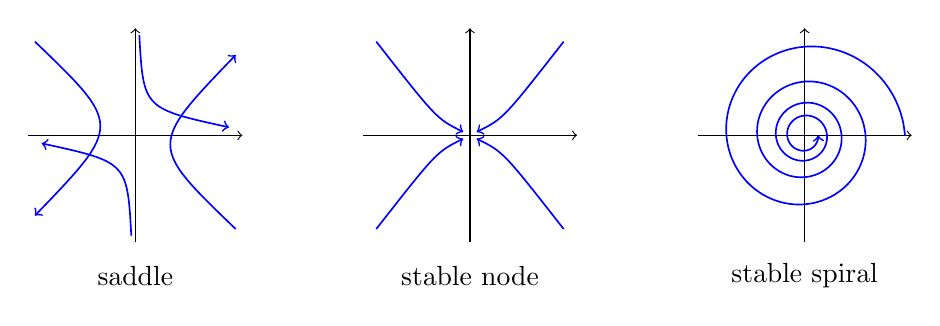
\begin{tikzpicture}[scale=0.85]
	% saddle
	\begin{scope}[shift={(-5,0)}]
		\draw [->] (-1.6, 0) -- (1.6, 0);
		\draw [->] (0, -1.6) -- (0, 1.6);
		\draw [blue, semithick, ->] (-1.5, 1.4) .. controls (-0.2, 0.15) .. (-1.5, -1.2) ;
		\draw [blue, semithick, ->] (1.5, -1.4) .. controls (0.2, -0.15) .. (1.5, 1.2);
		\draw [blue, semithick, ->] (0.06, 1.5) .. controls (0.12, 0.4) .. (1.4, 0.12);
		\draw [blue, semithick, ->] (-0.06, -1.5) .. controls (-0.12, -0.4) .. (-1.4, -0.12);
		\node at (0, -2.1) {saddle};
	\end{scope}
	% stable node
	\begin{scope}[shift={(0,0)}]
		\draw [->] (-1.6, 0) -- (1.6, 0);
		\draw [->] (0, -1.6) -- (0, 1.6);
		\draw [blue, semithick, ->] (1.4, 1.4) .. controls (0.5, 0.25) .. (0.1, 0.05);
		\draw [blue, semithick, ->] (-1.4, 1.4) .. controls (-0.5, 0.25) .. (-0.1, 0.05);
		\draw [blue, semithick, ->] (1.4, -1.4) .. controls (0.5, -0.25) .. (0.1, -0.05);
		\draw [blue, semithick, ->] (-1.4, -1.4) .. controls (-0.5, -0.25) .. (-0.1, -0.05);
		\node at (0, -2.1) {stable node};
	\end{scope}
	% spiral
	\begin{scope}[shift={(5,0)}]
		\draw [->] (-1.6, 0) -- (1.6, 0);
		\draw [->] (0, -1.6) -- (0, 1.6);
		\draw [blue, semithick, domain=0:1440, samples=200, smooth, variable=\t, ->]
			plot ({1.5*exp(-\t/720)*cos(\t)}, {1.5*exp(-\t/720)*sin(\t)});
		\node at (0, -2.1) {stable spiral};
	\end{scope}
\end{tikzpicture}
\end{center}

It is worth noting that everything here can be read off from just the trace and determinant of $M$, since $\lambda_1 \lambda_2 = \det M$ and $\lambda_1 + \lambda_2 = \tr M$: negative determinant means a saddle; positive determinant and negative trace a stable node or spiral (spiral if $(\tr M)^2 < 4 \det M$); and so on.

\begin{example}[The Damped Oscillator, Revisited]
	The damped oscillator $\ddot x + 2\kappa \dot x + x = 0$ from earlier becomes, upon setting $\vv Y = (x, \dot x)$, the planar system
	$$
	\dot{\vv Y} = \begin{pmatrix} 0 & 1 \\ -1 & -2\kappa \end{pmatrix} \vv Y,
	$$
	with $\tr M = -2\kappa$ and $\det M = 1$, so the eigenvalues are our old friends $\lambda = -\kappa \pm \sqrt{\kappa^2 - 1}$. Reading off the classification:
	\begin{itemize}
		\item $\kappa = 0$ (undamped): purely imaginary eigenvalues, a \emph{centre} -- the closed ellipses of simple harmonic motion in phase space, energy conserved.
		\item $0 < \kappa < 1$ (underdamped): complex eigenvalues with negative real part, a \emph{stable spiral} -- the trajectory winds around the origin as the oscillator swings back and forth, spiralling inwards as the amplitude decays.
		\item $\kappa > 1$ (overdamped): two negative real eigenvalues, a \emph{stable node} -- no more winding; trajectories slide into the origin, tangent to the slow eigenvector.
	\end{itemize}
	The transition through critical damping $\kappa = 1$ is precisely the moment the spiral degenerates into a node, i.e.\ the eigenvalues collide on the real axis. Phase-portrait language and the earlier time-domain analysis are two views of the same underlying picture.
\end{example}

\begin{example}[An Initial Value Problem]
	Continuing the earlier example, let's impose the initial condition $\vv Y(0) = (0, 0)$ on
	$$
	\vv Y = A \begin{pmatrix} 4 \\ 1 \end{pmatrix} e^{2t} + B \begin{pmatrix} -6 \\ 1 \end{pmatrix} e^{-8t} - \begin{pmatrix} 4 \\ 1 \end{pmatrix} e^t.
	$$
	At $t = 0$:
	$$
	4A - 6B - 4 = 0, \qquad A + B - 1 = 0,
	$$
	so $B = 1 - A$ and $4A - 6 + 6A = 4$, giving $A = 1$, $B = 0$. The solution through the origin is
	$$
	\vv Y = \begin{pmatrix} 4 \\ 1\end{pmatrix}\left(e^{2t} - e^t\right):
	$$
	as it happens the $e^{-8t}$ mode is not excited at all, and this particular trajectory runs along the fixed direction $(4, 1)$ for all time.
\end{example}

\subsection{Nonlinear Systems and Linearisation}

Finally we come to nonlinear autonomous systems,
$$
\dot x = f(x, y), \qquad \dot y = g(x, y),
$$
where $f$ and $g$ have no explicit time-dependence. Solving such systems exactly is usually hopeless, but -- just as for single autonomous equations -- we can understand the phase portrait by finding the equilibria and analysing the flow near each.

\begin{definition}[Equilibrium Point of a System]
	An \vocab{equilibrium point} of the system is a point $(x_0, y_0)$ where $\dot x = \dot y = 0$, i.e.\ where $f(x_0, y_0) = g(x_0, y_0) = 0$ simultaneously.
\end{definition}

Near an equilibrium, write $x = x_0 + \xi$, $y = y_0 + \eta$ for small perturbations $\xi, \eta$, and Taylor expand:
$$
\dot \xi = f(x_0 + \xi, y_0 + \eta) = \underbrace{f(x_0, y_0)}_{=0} + \xi f_x + \eta f_y + O(\xi^2, \xi\eta, \eta^2),
$$
and similarly for $\dot\eta$. Dropping the quadratic terms, we obtain the \vocab{linearised system}
$$
\begin{pmatrix} \dot \xi \\ \dot \eta \end{pmatrix} = \begin{pmatrix} f_x & f_y \\ g_x & g_y \end{pmatrix}\begin{pmatrix} \xi \\ \eta \end{pmatrix},
$$
where the matrix of partial derivatives (the \emph{Jacobian}) is evaluated at the equilibrium. This is a linear system of exactly the type we have just classified, so near each equilibrium the phase portrait looks (in the non-degenerate cases) like a saddle, node or spiral, determined by the Jacobian's eigenvalues. The global phase portrait is then assembled by patching together these local pictures.

\begin{example}[A Predator--Prey System]
	Suppose $x(t)$ counts prey and $y(t)$ predators. A reasonable model:
	$$
	\dot x = \underbrace{\alpha x}_{\text{births}} - \underbrace{\beta x^2}_{\text{competition}} - \underbrace{\gamma xy}_{\text{predation}}, \qquad
	\dot y = \underbrace{\varepsilon xy}_{\text{food supply}} - \underbrace{\delta y}_{\text{deaths}}.
	$$
	Take, concretely,
	$$
	\dot x = 8x - 2x^2 - 2xy, \qquad \dot y = xy - y.
	$$
	\emph{Equilibria.} We need $x(8 - 2x - 2y) = 0$ and $y(x - 1) = 0$. The first gives $x = 0$ or $y = 4 - x$; the second gives $y = 0$ or $x = 1$. Combining, the equilibria are
	$$
	(0, 0), \qquad (4, 0), \qquad (1, 3).
	$$

	\emph{Near $(0,0)$.} The linearisation is
	$$
	\begin{pmatrix} \dot\xi \\ \dot\eta \end{pmatrix} = \begin{pmatrix} 8 & 0 \\ 0 & -1 \end{pmatrix}\begin{pmatrix} \xi \\ \eta\end{pmatrix},
	$$
	with eigenvalues $8, -1$ along the coordinate axes: a \emph{saddle}, unstable along the prey axis (a few prey with no predators multiply) and stable along the predator axis (predators with no prey starve).

	\emph{Near $(4, 0)$.} Set $x = 4 + \xi$, $y = \eta$. Rather than computing the Jacobian abstractly, we can substitute directly and discard quadratic terms:
	\begin{align*}
		\dot \xi &= (4 + \xi)(8 - 8 - 2\xi - 2\eta) = -8\xi - 8\eta + O(2), \\
		\dot \eta &= \eta(4 + \xi - 1) = 3\eta + O(2).
	\end{align*}
	The matrix $\begin{pmatrix} -8 & -8 \\ 0 & 3 \end{pmatrix}$ has eigenvalues $-8$ and $3$ (it is triangular), with eigenvectors $(1, 0)$ and $(8, -11)$: another \emph{saddle}. A prey-only population at carrying capacity is unstable to the introduction of predators.

	\emph{Near $(1, 3)$.} Set $x = 1 + \xi$, $y = 3 + \eta$:
	\begin{align*}
		\dot\xi &= (1 + \xi)(8 - 2 - 2\xi - 6 - 2\eta) \approx -2\xi - 2\eta, \\
		\dot\eta &= (3 + \eta)\xi \approx 3\xi.
	\end{align*}
	The matrix $\begin{pmatrix} -2 & -2 \\ 3 & 0\end{pmatrix}$ has characteristic equation $\lambda^2 + 2\lambda + 6 = 0$, giving
	$$
	\lambda = -1 \pm i \sqrt 5.
	$$
	Complex with negative real part: a \emph{stable spiral}. To find the sense of rotation, perturb to the right, $(\xi, \eta) = (\xi, 0)$ with $\xi > 0$: then $(\dot \xi, \dot\eta) = (-2\xi, 3\xi)$, pointing up and to the left, so the spiral is anticlockwise.

	\emph{The global picture.} Patching the three local portraits together: trajectories leave the two saddles along their unstable directions and are drawn into the spiral. Almost every solution with $x, y > 0$ spirals in towards the coexistence state $(1, 3)$ -- predators and prey settle down, through decaying oscillations, to stable coexistence.
\end{example}

\section{Partial Differential Equations}

We end the course with a first look at \emph{partial} differential equations -- equations involving partial derivatives of a function of several variables. The subject is vast (much of IB and beyond is devoted to it), but even with the tools we already have, we can solve some of the most important examples: the wave equation and the diffusion equation.

\subsection{The First-Order Wave Equation}

Consider, for a function $y(x, t)$ and a constant $c$, the equation
$$
\frac{\partial y}{\partial t} = c \frac{\partial y}{\partial x},
$$
known as the \vocab{first-order wave equation}. The key idea for solving it -- the \vocab{method of characteristics} -- is to stop thinking of $y$ as a function on the whole $(x, t)$ plane, and instead watch how $y$ varies along well-chosen \emph{paths} $x = x(t)$.

Along a path $x(t)$, the multivariate chain rule gives
$$
\frac{\mathrm{d}}{\mathrm{d}t} y(x(t), t) = \frac{\partial y}{\partial t} + \frac{\mathrm{d}x}{\mathrm{d}t}\frac{\partial y}{\partial x} = \left(c + \frac{\mathrm{d}x}{\mathrm{d}t}\right)\frac{\partial y}{\partial x},
$$
where we used the PDE in the last step. Now \emph{choose} the paths to kill the right-hand side: along paths with
$$
\frac{\mathrm{d}x}{\mathrm{d}t} = -c \qquad \text{we have} \qquad \frac{\mathrm{d}y}{\mathrm{d}t} = 0.
$$
We have traded one PDE for a pair of ODEs. The chosen paths, called the \vocab{characteristics} of the equation, are the straight lines $x = x_0 - ct$, one for each constant $x_0 = x + ct$; and along each characteristic, $y$ is constant. So the value of $y$ at $(x,t)$ depends only on which characteristic the point lies on -- that is, only on $x + ct$:
$$
y = f(x + ct)
$$
for an arbitrary function $f$ (one can check directly that any such $y$ solves the equation). This is a \emph{wave}: the profile $f$ translates rigidly to the left with speed $c$, unchanged in shape. Note that in place of the arbitrary \emph{constants} in the general solutions of ODEs, the general solution of a PDE contains an arbitrary \emph{function}.

It is helpful to picture the characteristics in the $(x, t)$ plane: a family of parallel lines of slope $-1/c$, each carrying a single constant value of $y$, transported up from its intersection with the $x$-axis.

\begin{center}
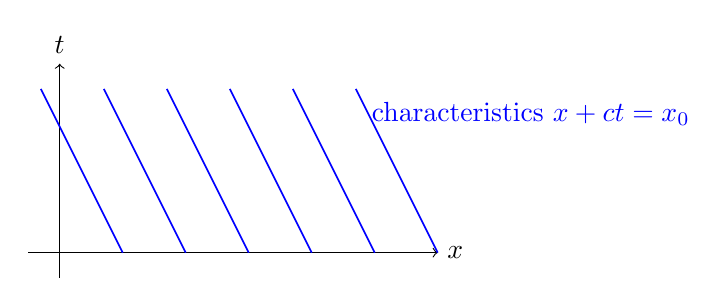
\begin{tikzpicture}[scale=0.8]
	\draw [->] (-0.5, 0) -- (6, 0) node [right] {$x$};
	\draw [->] (0, -0.4) -- (0, 3) node [above] {$t$};
	\foreach \x in {1, 2, 3, 4, 5, 6} {
		\draw [blue, semithick] (\x, 0) -- (\x - 1.3, 2.6);
	}
	\node [blue, right] at (4.8, 2.2) {characteristics $x + ct = x_0$};
\end{tikzpicture}
\end{center}

The arbitrary function is pinned down by initial data. Given $y(x, 0)$, we have $f(x) = y(x, 0)$ and hence the full solution: to find $y$ at $(x, t)$, follow the characteristic through that point back down to the $x$-axis and read off the initial value there.

\begin{example}
	Solve $y_t = c y_x$ with $y(x, 0) = x^2 - 3$. Since $y = f(x + ct)$ with $f(x) = x^2 - 3$,
	$$
	y = (x + ct)^2 - 3,
	$$
	the initial parabola sliding left at speed $c$.
\end{example}

Forced versions succumb to the same method -- along the characteristics, $y$ is no longer constant, but satisfies an ODE we can solve.

\begin{example}
	Solve
	$$
	\frac{\partial y}{\partial t} + 5 \frac{\partial y}{\partial x} = e^{-t}, \qquad y(x, 0) = e^{-x^2}.
	$$
	The characteristics are now $\frac{\mathrm{d}x}{\mathrm{d}t} = 5$, i.e.\ the lines $x_0 = x - 5t$, and along them
	$$
	\frac{\mathrm{d}y}{\mathrm{d}t} = e^{-t} \implies y = F(x_0) - e^{-t},
	$$
	with a `constant of integration' $F(x_0)$ that may differ from characteristic to characteristic. At $t = 0$ we have $x = x_0$ and $y = F(x_0) - 1 = e^{-x_0^2}$, so $F(x_0) = 1 + e^{-x_0^2}$, and
	$$
	y = 1 + e^{-(x - 5t)^2} - e^{-t}.
	$$
	A rightward-travelling Gaussian pulse, riding on a background that relaxes from $0$ up to $1$.
\end{example}

\subsection{The Second-Order Wave Equation}

The equation usually called \emph{the} wave equation is second order:
$$
\frac{\partial^2 y}{\partial t^2} = c^2 \frac{\partial^2 y}{\partial x^2}.
$$
This models, for instance, small transverse vibrations of a taut string, with $y(x, t)$ the displacement at position $x$ and time $t$: the acceleration of each element of string is proportional to the local \emph{curvature} $y_{xx}$, since a straight (even sloped) string feels no net sideways force, while a curved one does.

To solve it, factorise the differential operator:
$$
\frac{\partial^2}{\partial t^2} - c^2 \frac{\partial^2}{\partial x^2} = \left(\frac{\partial}{\partial t} - c \frac{\partial}{\partial x}\right)\left(\frac{\partial}{\partial t} + c\frac{\partial}{\partial x}\right),
$$
where the two first-order factors commute. Anything annihilated by either factor is annihilated by the product, and each factor is a first-order wave equation, solved above. So $y = f(x + ct)$ and $y = g(x - ct)$ are both solutions, and by linearity so is their sum. In fact this is everything:

\begin{proposition}[d'Alembert's Solution]
	The general solution of $y_{tt} = c^2 y_{xx}$ is
	$$
	y = f(x + ct) + g(x - ct)
	$$
	for arbitrary (twice-differentiable) functions $f$ and $g$: a superposition of a leftward- and a rightward-travelling wave, each moving at speed $c$ with fixed profile.
\end{proposition}
\begin{proof}
	That these are solutions is a direct check. For the converse, change variables to $\xi = x + ct$ and $\eta = x - ct$; the chain rule turns the equation into
	$$
	y_{tt} - c^2 y_{xx} = -4c^2 \frac{\partial^2 y}{\partial \xi \, \partial \eta} = 0,
	$$
	and integrating once in each variable gives $y = f(\xi) + g(\eta)$.
\end{proof}

Since the equation is second order in $t$ (and in $x$), we expect to need two initial conditions and two boundary conditions to pin down a unique solution -- one pair for each of the two arbitrary functions.

\begin{example}
	Solve $y_{tt} = c^2 y_{xx}$ subject to
	$$
	y(x, 0) = \frac{1}{1 + x^2}, \qquad y_t(x, 0) = 0, \qquad y \to 0 \text{ as } x \to \pm\infty.
	$$
	Write $y = f(x + ct) + g(x - ct)$. The initial conditions give
	$$
	f(x) + g(x) = \frac{1}{1 + x^2}, \qquad c f'(x) - c g'(x) = 0.
	$$
	The second says $f' = g'$, so $f = g + A$ for a constant $A$; since only $f + g$ enters the solution, we may absorb the constant and take $f = g$, whence
	$$
	f(x) = g(x) = \frac{1}{2(1 + x^2)},
	$$
	and
	$$
	y = \frac{1}{2}\left[\frac{1}{1 + (x + ct)^2} + \frac{1}{1 + (x - ct)^2}\right].
	$$
	The initial hump splits into two half-height copies, travelling apart at speeds $\pm c$.
\end{example}

\subsection{The Diffusion Equation}

Our final equation models heat conduction in one dimension. If $T(x, t)$ is the temperature in a solid bar, then
$$
\frac{\partial T}{\partial t} = \kappa \frac{\partial^2 T}{\partial x^2},
$$
where the constant $\kappa > 0$ is the \vocab{diffusivity}. This is the \vocab{diffusion equation} (or heat equation). Structurally it looks like the wave equation with one time derivative removed, and this changes the character of solutions completely: for the wave equation, curvature drives \emph{acceleration} and disturbances propagate forever; here, curvature drives \emph{velocity}, so bumps in the temperature profile simply flatten themselves out. Diffusion is dissipative, not oscillatory.

\begin{remark}[Nomenclature]
	Second-order linear PDEs are traditionally classified by loose analogy with conic sections: the wave equation $y_{tt} - c^2 y_{xx} = 0$ is called \emph{hyperbolic} (compare $t^2 - c^2x^2 = \text{const}$), the diffusion equation is \emph{parabolic} ($t = x^2$-like, one time derivative against two space derivatives), and Laplace's equation $y_{xx} + y_{yy} = 0$, which the reader will meet in Vector Calculus, is \emph{elliptic}. The analogy is purely formal, but the classification is genuinely meaningful: hyperbolic equations propagate signals along characteristics, parabolic ones smooth and dissipate, and elliptic ones describe equilibrium states.
\end{remark}

We will solve one classic problem, which also introduces the useful idea of a \emph{similarity solution}.

\begin{example}[Heating a Semi-Infinite Bar]
	Consider an infinitely long bar occupying $x \geq 0$, initially cold, whose end $x = 0$ is abruptly heated to unit temperature at $t = 0$ and held there:
	$$
	T(x, 0) = 0, \qquad T(0, t) = H(t), \qquad T(x, t) \to 0 \text{ as } x \to \infty,
	$$
	where $H$ is the Heaviside function.

	The key observation is dimensional. The only parameter in the problem is $\kappa$, with dimensions $(\text{length})^2/(\text{time})$, and neither the initial nor boundary data introduces any length scale. So the only dimensionless combination of $x$ and $t$ available is
	$$
	\eta = \frac{x}{2\sqrt{\kappa t}}
	$$
	(the factor $2$ is for later convenience), and it is natural to seek a \vocab{similarity solution} depending on $x$ and $t$ only through $\eta$:
	$$
	T(x, t) = \theta(\eta).
	$$
	The temperature profiles at different times should all be the same shape, stretched horizontally by $\sqrt{\kappa t}$. Let's compute the derivatives by the chain rule:
	\begin{align*}
		\frac{\partial T}{\partial x} &= \theta'(\eta) \frac{\partial \eta}{\partial x} = \frac{1}{2\sqrt{\kappa t}}\theta'(\eta), \qquad
		\frac{\partial^2 T}{\partial x^2} = \frac{1}{4 \kappa t} \theta''(\eta), \\
		\frac{\partial T}{\partial t} &= \theta'(\eta) \frac{\partial \eta}{\partial t} = -\frac{1}{2} \cdot \frac{x}{2\sqrt{\kappa}\, t^{3/2}} \theta'(\eta) = -\frac{\eta}{2t}\theta'(\eta).
	\end{align*}
	Substituting into the PDE:
	$$
	-\frac{\eta}{2t} \theta' = \frac{1}{4t}\theta'' \implies \theta'' + 2\eta \, \theta' = 0.
	$$
	All the $x$'s and $t$'s have vanished, leaving an ODE for $\theta(\eta)$ -- the sign that our similarity guess was consistent. Moreover it is an ODE we can solve: it is first order in $\theta'$, with integrating factor $\mu = \exp(\int 2\eta \dd\eta) = e^{\eta^2}$, so
	$$
	\left(e^{\eta^2} \theta'\right)' = 0 \implies \theta' = A e^{-\eta^2} \implies \theta = A \int_0^\eta e^{-u^2} \dd u + B.
	$$
	This integral has a standard name: the \emph{error function} $\operatorname{erf}(\eta) = \frac{2}{\sqrt\pi} \int_0^\eta e^{-u^2} \dd u$, normalised so that $\operatorname{erf}(\eta) \to 1$ as $\eta \to \infty$. So $\theta = \alpha \operatorname{erf}(\eta) + B$.

	Now the boundary conditions, translated into $\eta$: the heated end $x = 0$ (with $t > 0$) corresponds to $\eta = 0$, so $\theta(0) = 1$, giving $B = 1$. The far field $x \to \infty$ (or the initial instant $t \to 0^+$) corresponds to $\eta \to \infty$, so $\theta(\infty) = 0$, giving $\alpha = -1$. Hence $\theta = 1 - \operatorname{erf}(\eta)$, and
	$$
	T(x, t) = \operatorname{erfc}\left(\frac{x}{2 \sqrt{\kappa t}}\right),
	$$
	where $\operatorname{erfc} = 1 - \operatorname{erf}$ is the complementary error function.

	The physical picture: at each time $t$, the temperature falls smoothly from $1$ at the hot end towards $0$, over a penetration depth of order $\sqrt{\kappa t}$. Heat creeps into the bar with the characteristic square-root-of-time spreading of diffusion -- to heat twice as deep takes four times as long. (This also tells us when a \emph{finite} bar of length $L$ can be treated as infinite: precisely when $\sqrt{\kappa t} \ll L$, i.e.\ $t \ll L^2/\kappa$.)
\end{example}

And that is where we stop. We have seen equations solved exactly, approximated, discretised, linearised and sketched; the recurring themes -- eigenfunctions, linearity, superposition, equilibria, stability -- will reappear throughout the rest of the Tripos, in Methods and Analysis and far beyond. Differential equations are never really finished; one simply stops.

\end{document}
